  \documentclass[final]{beamer} % beamer 3.10: do NOT use option hyperref={pdfpagelabels=false} !
%\documentclass[final,hyperref={pdfpagelabels=false}]{beamer} % beamer 3.07: get rid of beamer warnings
\mode<presentation> {  %% check http://www-i6.informatik.rwth-aachen.de/~dreuw/latexbeamerposter.php for examples
	\usetheme{prometheus}    %% you should define your own theme e.g. for big headlines using your own logos
}
\setbeamertemplate{caption}[numbered]

\usepackage[english]{babel}
\usepackage[latin1]{inputenc}
\usepackage{amsmath,amsthm, amssymb, latexsym}
%\usepackage{times}\usefonttheme{professionalfonts}  % times is obsolete
\usefonttheme[onlymath]{serif}
\boldmath
\usepackage[orientation=landscape,size=a1,debug]{beamerposter}
\usepackage{float}    
\usepackage{subcaption}              % e.g. for DIN-A0 poster
%\usepackage[orientation=portrait,size=a1,scale=1.4,grid,debug]{beamerposter}                  % e.g. for DIN-A1 poster, with optional grid and debug output
%\usepackage[size=custom,width=200,height=120,scale=2,debug]{beamerposter}                     % e.g. for custom size poster
%\usepackage[orientation=portrait,size=a0,scale=1.0,printer=rwth-glossy-uv.df]{beamerposter}   % e.g. for DIN-A0 poster with rwth-glossy-uv printer check
% ...
%
\title[Fancy Posters]{Prometheus AI}
\author{Sean Stappas --- Supervised by Prof. Vybihal}
\institute[RWTH Aachen University]{}
\date{Jul. 31th, 2007}

% edit this depending on how tall your header is. We should make this scaling automatic :-/
\newlength{\columnheight}
\setlength{\columnheight}{100cm}

\begin{document}
	\begin{frame}
		\begin{columns}
			\begin{column}{.3\textwidth}
				\parbox[t][\columnheight]{\textwidth}{
				\begin{block}{Introduction}
					\begin{itemize}
						\item Prometheus
						\begin{itemize}
							\item Model of the human brain.
							\item Controls multiple robots in a swarm.
						\end{itemize}
					\end{itemize}
				
					\begin{figure}[!htb]
						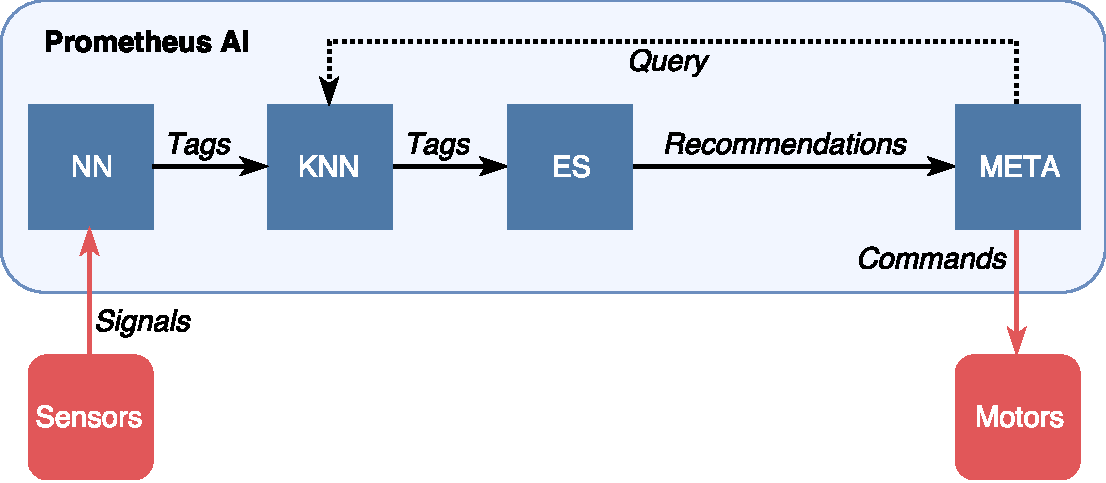
\includegraphics[width=0.7\textwidth]{figures/ai_model_labeled.pdf}
						\caption{Prometheus AI model with labeled input and output.}
						\label{model_labeled}
					\end{figure}
						
					\begin{itemize}
						\item Neural Netowrk (NN)
						\begin{itemize}
							\item Low-level signal processor.
						\end{itemize}
					\end{itemize}
					
					\begin{itemize}
						\item Knowledge Node Network (KNN)
						\begin{itemize}
							\item Represents memory.
						\end{itemize}
					\end{itemize}
					
					\begin{figure}[!htb]
						\centering
						\begin{subfigure}[!htb]{0.4\columnwidth}
							\centering
							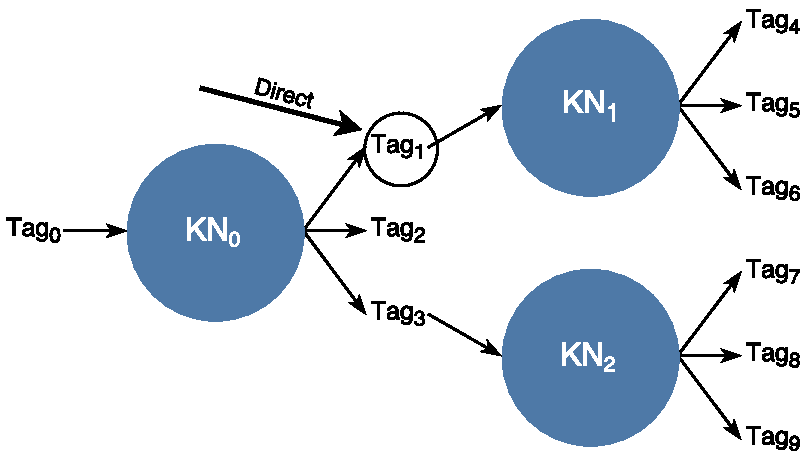
\includegraphics[height=2in]{figures/direct_search.pdf}
							\caption{Direct searching.}
						\end{subfigure}
						\quad
						\begin{subfigure}[!htb]{0.4\columnwidth}
							\centering
							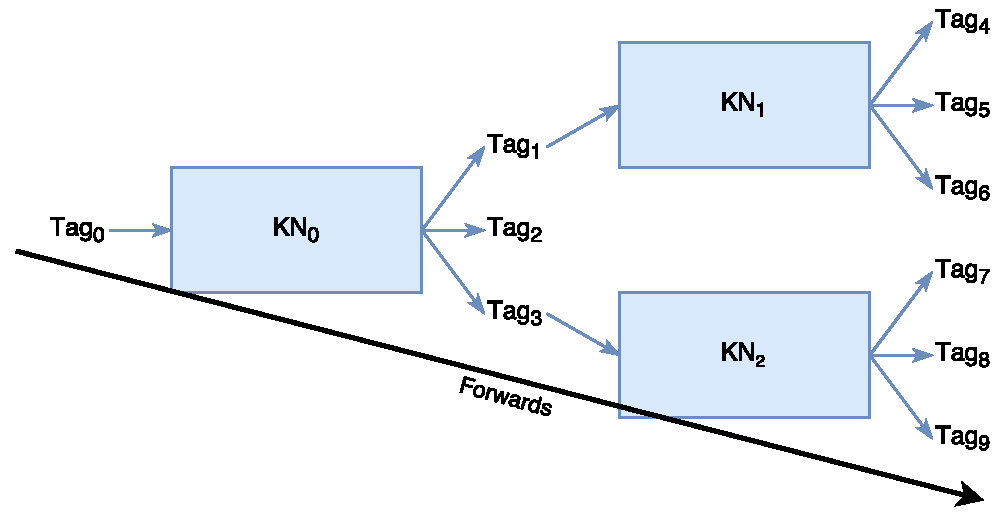
\includegraphics[height=2in]{figures/forwards_thinking.pdf}
							\caption{Forward searching/thinking.}
							\label{think_forwards}
						\end{subfigure}
						\bigskip
						\begin{subfigure}[!htb]{0.4\columnwidth}
							\centering
							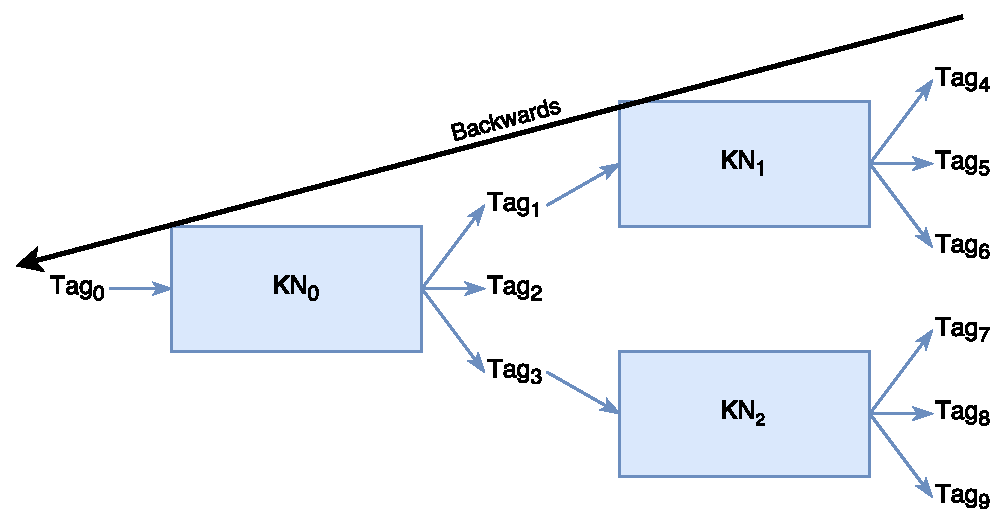
\includegraphics[height=2.1in]{figures/backwards_thinking.pdf}
							\caption{Backward searching/thinking.}
							\label{think_backwards}
						\end{subfigure}
						~
						\begin{subfigure}[!htb]{0.4\columnwidth}
							\centering
							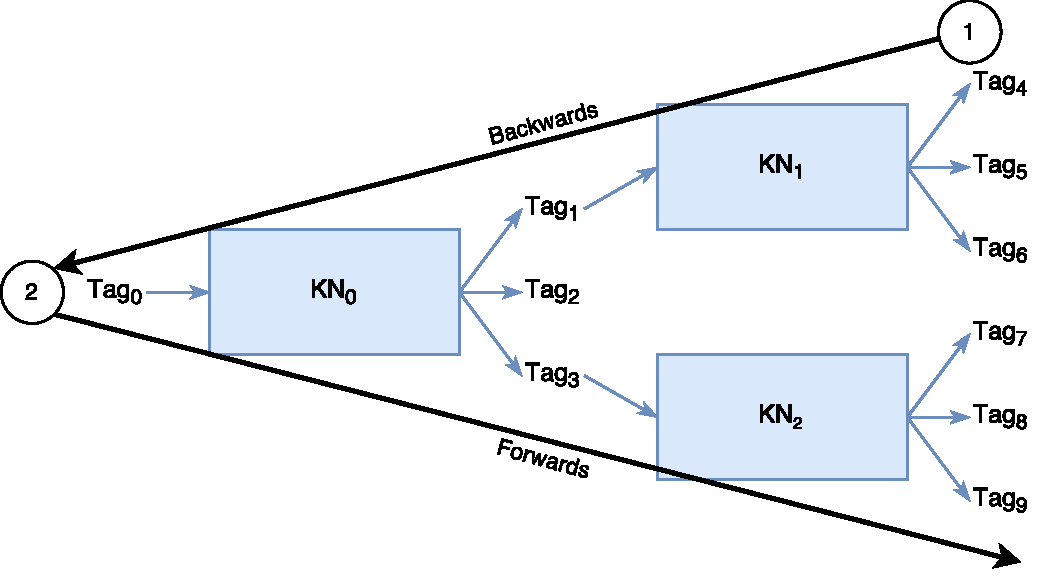
\includegraphics[height=2.1in]{figures/lambda_thinking.pdf}
							\caption{Lambda searching/thinking.}
							\label{think_lambda}
						\end{subfigure}
						\caption{Methods of searching and thinking in the KNN.}
					\end{figure}
					
					\begin{itemize}
						\item Expert System (ES)
						\begin{itemize}
							\item Logical reasoner.
							\item Unaware of context.
						\end{itemize}
					\end{itemize}
					
					\begin{table}[!htb]
						\centering
						\caption{Fact predicates in the ES.}
						\begin{tabular}{r | l}
							\textbf{Fact} & \textbf{Meaning} \\ \hline
							$(A)$ & $A$ is true or active.\\
							$(A = 1)$ & $A$ is equal to 1. \\
							$(A > 1)$ & $A$ is greater than 1. \\
							$(A \ ?)$ & $A$ can take any value.
						\end{tabular}
						\label{table:fact_predicates}
					\end{table}
					
					\begin{equation} \label{eq:rule}
					Fact_1 \cdots Fact_m \rightarrow Tag_1 \cdots Tag_n
					\end{equation}
					
					\begin{itemize}
						\item Meta Reasoner (META)
						\begin{itemize}
							\item High-level decision-maker.
						\end{itemize}
					\end{itemize}
				
				\end{block}
				\begin{block}{Problem}
				\begin{itemize}
					\item Design and implement the ES and KNN in Java.
					\begin{itemize}
						\item Create an initial design.
						\item Build a code skeleton.
						\item Implement integration and unit tests.
					\end{itemize}
				
					\item Supervise undergraduate students working on Prometheus.
					\begin{itemize}
						\item Provide resources.
						\item Review code.
					\end{itemize}
				\end{itemize}
				\end{block}
			}
			\end{column}
			\begin{column}{.35\textwidth}
				\parbox[t][\columnheight]{\textwidth}{
				\begin{block}{Design \& Implementation}
					\begin{itemize}
						\item Dependencies modeled using Google Guice.
						\begin{itemize}
							\item Framework for modular dependency injection.
							\item Allows for easily testable code.
						\end{itemize}
					\end{itemize}
					
					\begin{figure}[!htb]
						\centering
						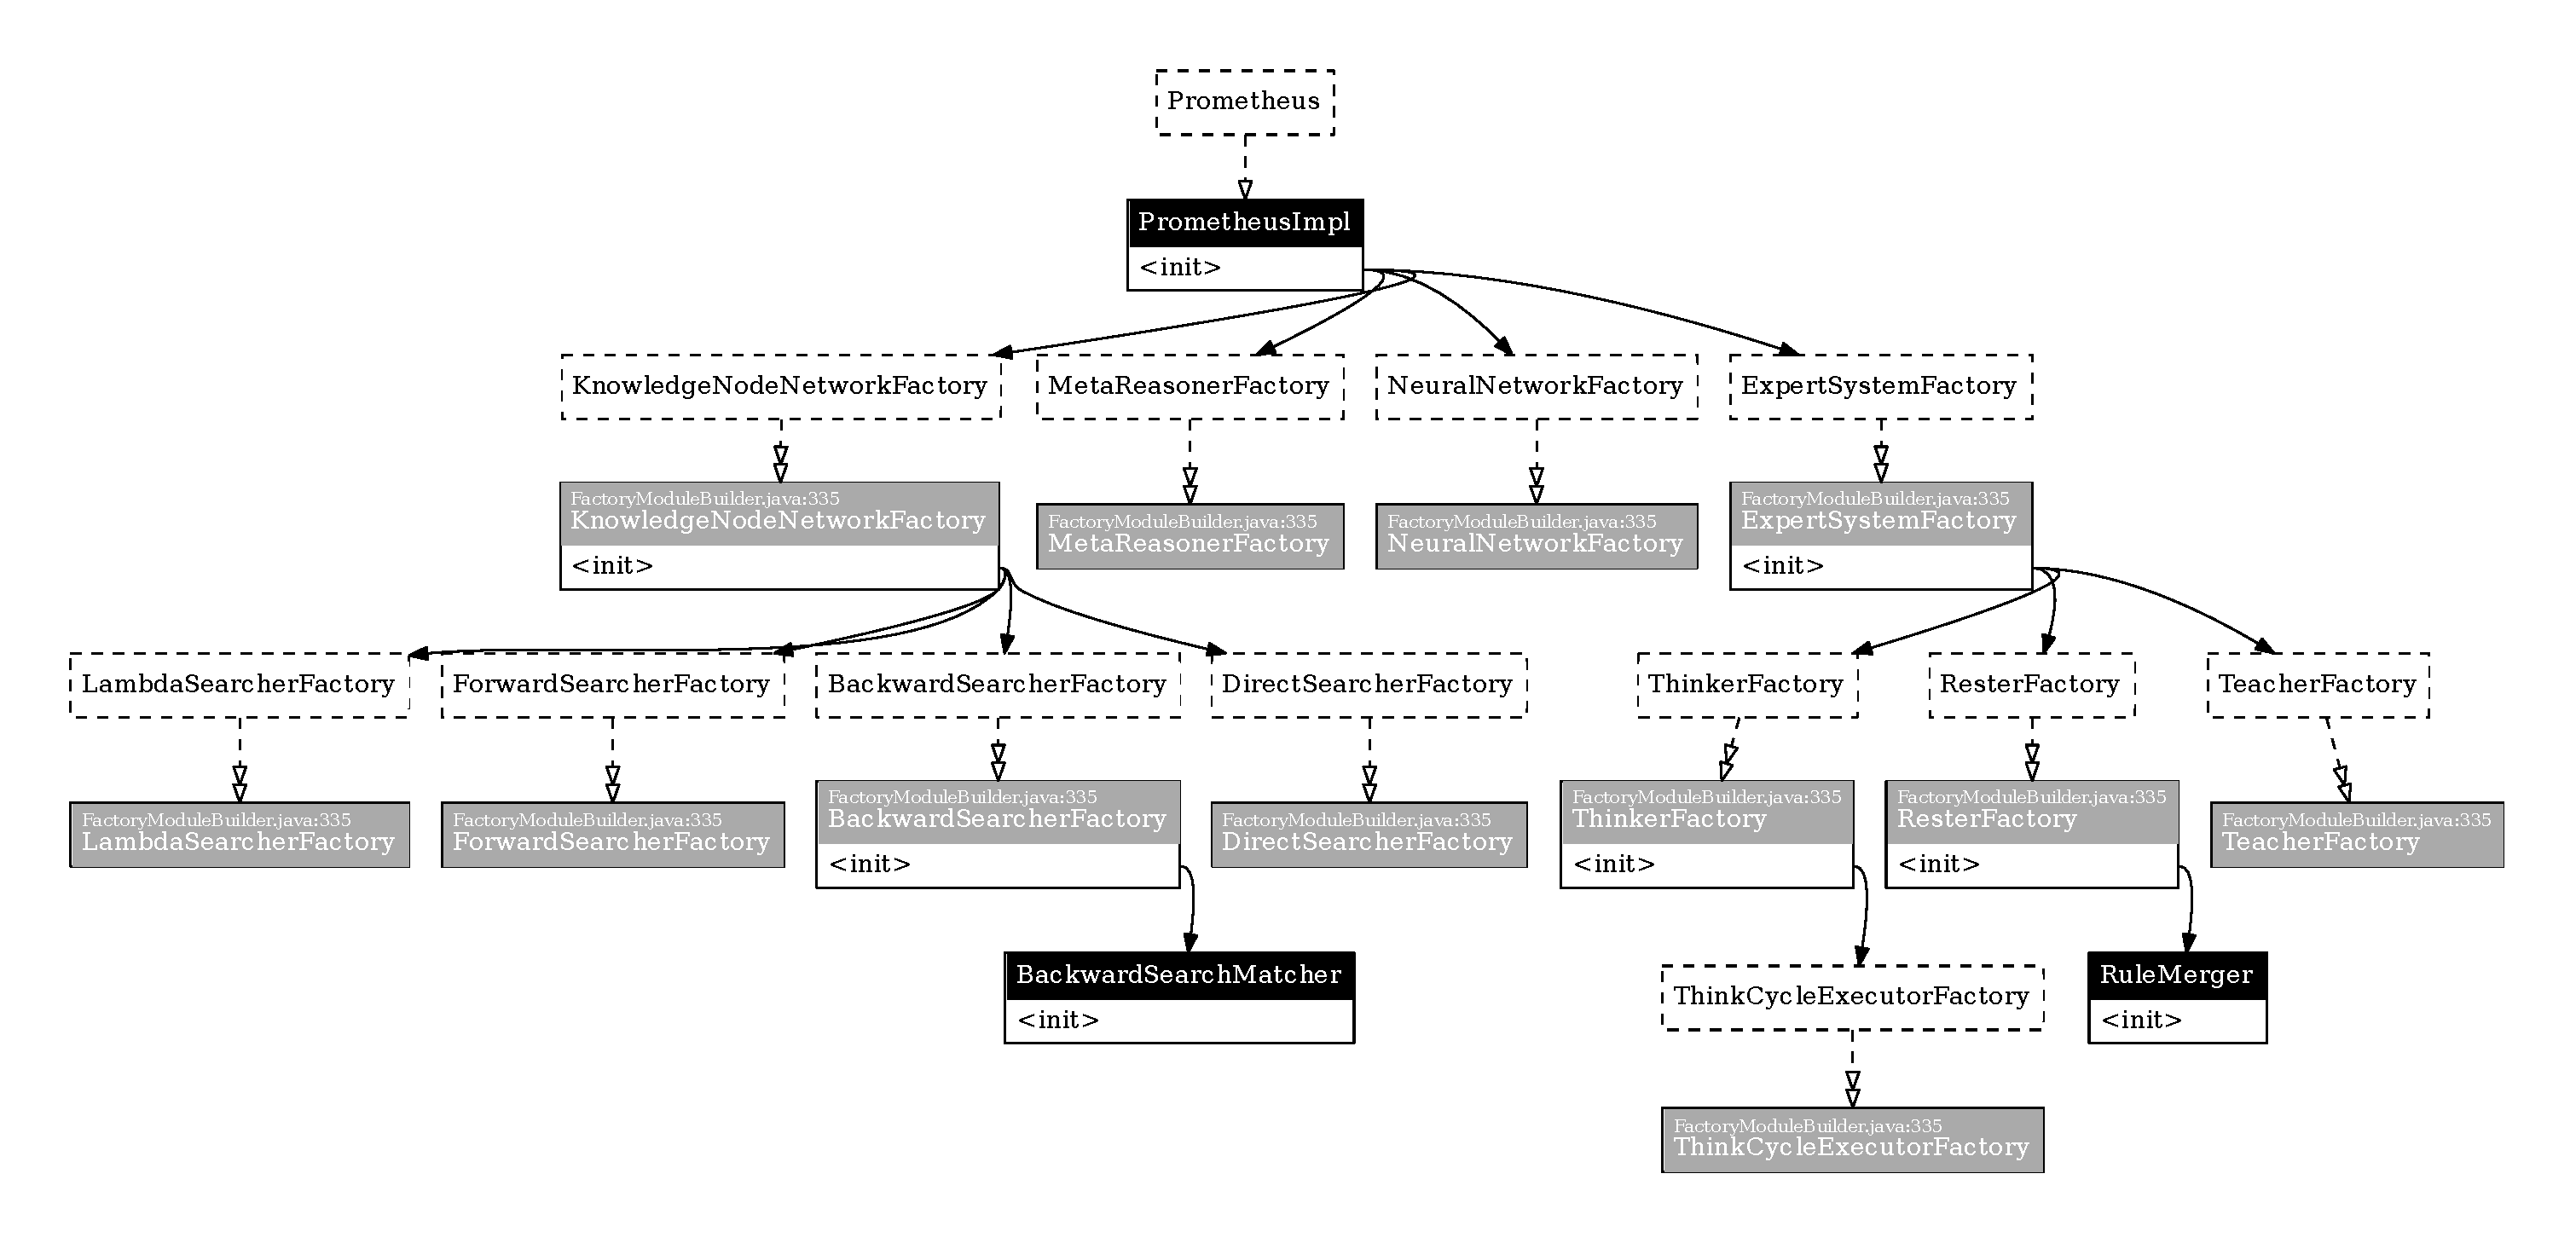
\includegraphics[width=\columnwidth]{figures/guice_graph.pdf}
						\caption
						{Guice dependency graph.}
					\end{figure}
					
					\begin{itemize}
						\item Tag object is central to the ES and KNN.
						\begin{itemize}
							\item Represents a unit of information.
							\item Can be instantiated as Fact, Rule or Recommendation classes.
						\end{itemize}
					\end{itemize}
				
					\begin{figure}[!htb]
						\centering
						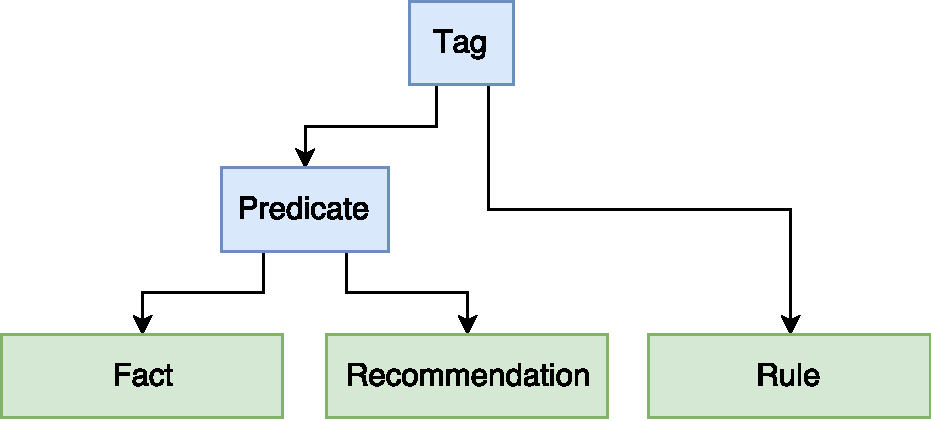
\includegraphics[width=0.5\columnwidth]{figures/prometheus_tags.pdf}
						\caption
						{Tag inheritance graph.}
					\end{figure}
					
%					\begin{figure}[!htb]
%						\centering
%						%			\begin{subfigure}[!htb]{0.3\textwidth}
%						%				\centering
%						%				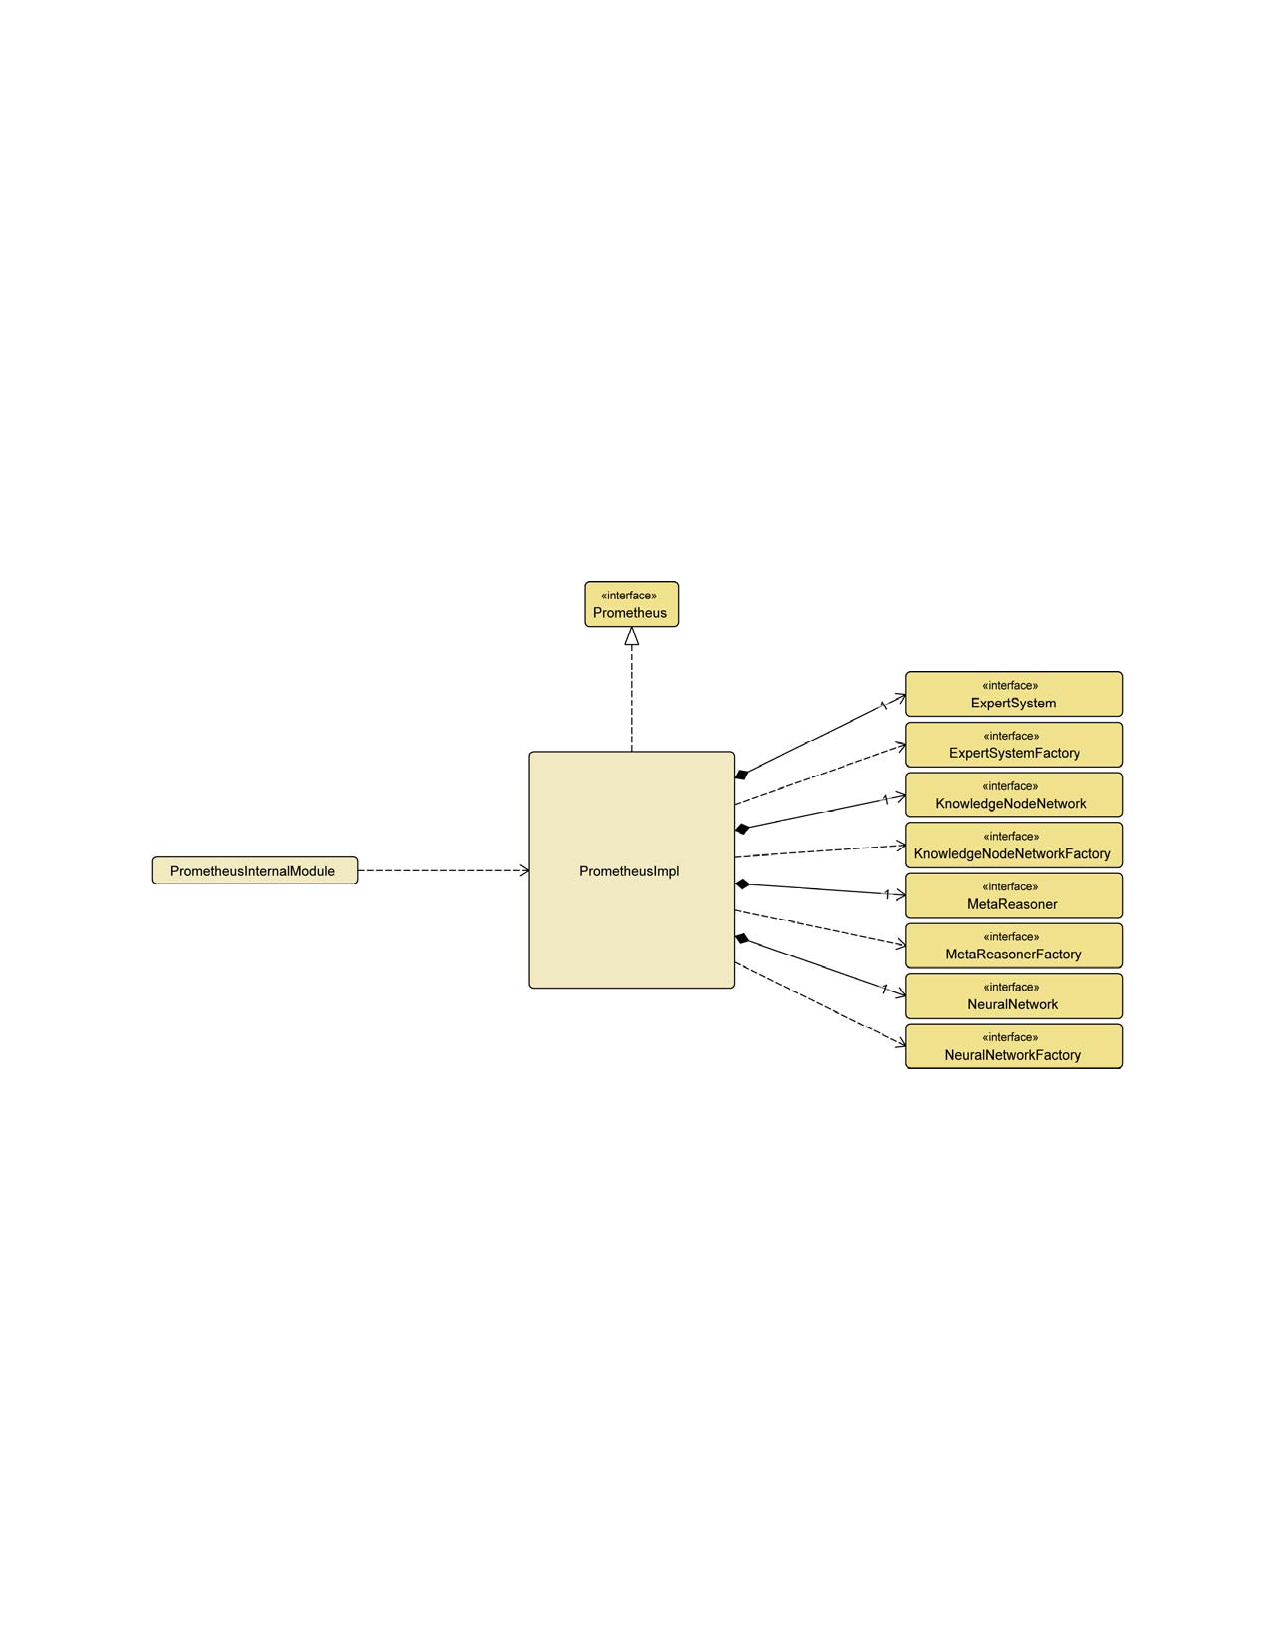
\includegraphics[width=\textwidth]{figures/prometheus_uml.pdf}
%						%				\caption
%						%				{Prometheus package.}
%						%			\end{subfigure}
%						%			~
%						\begin{subfigure}[!htb]{0.4\columnwidth}
%							\centering
%							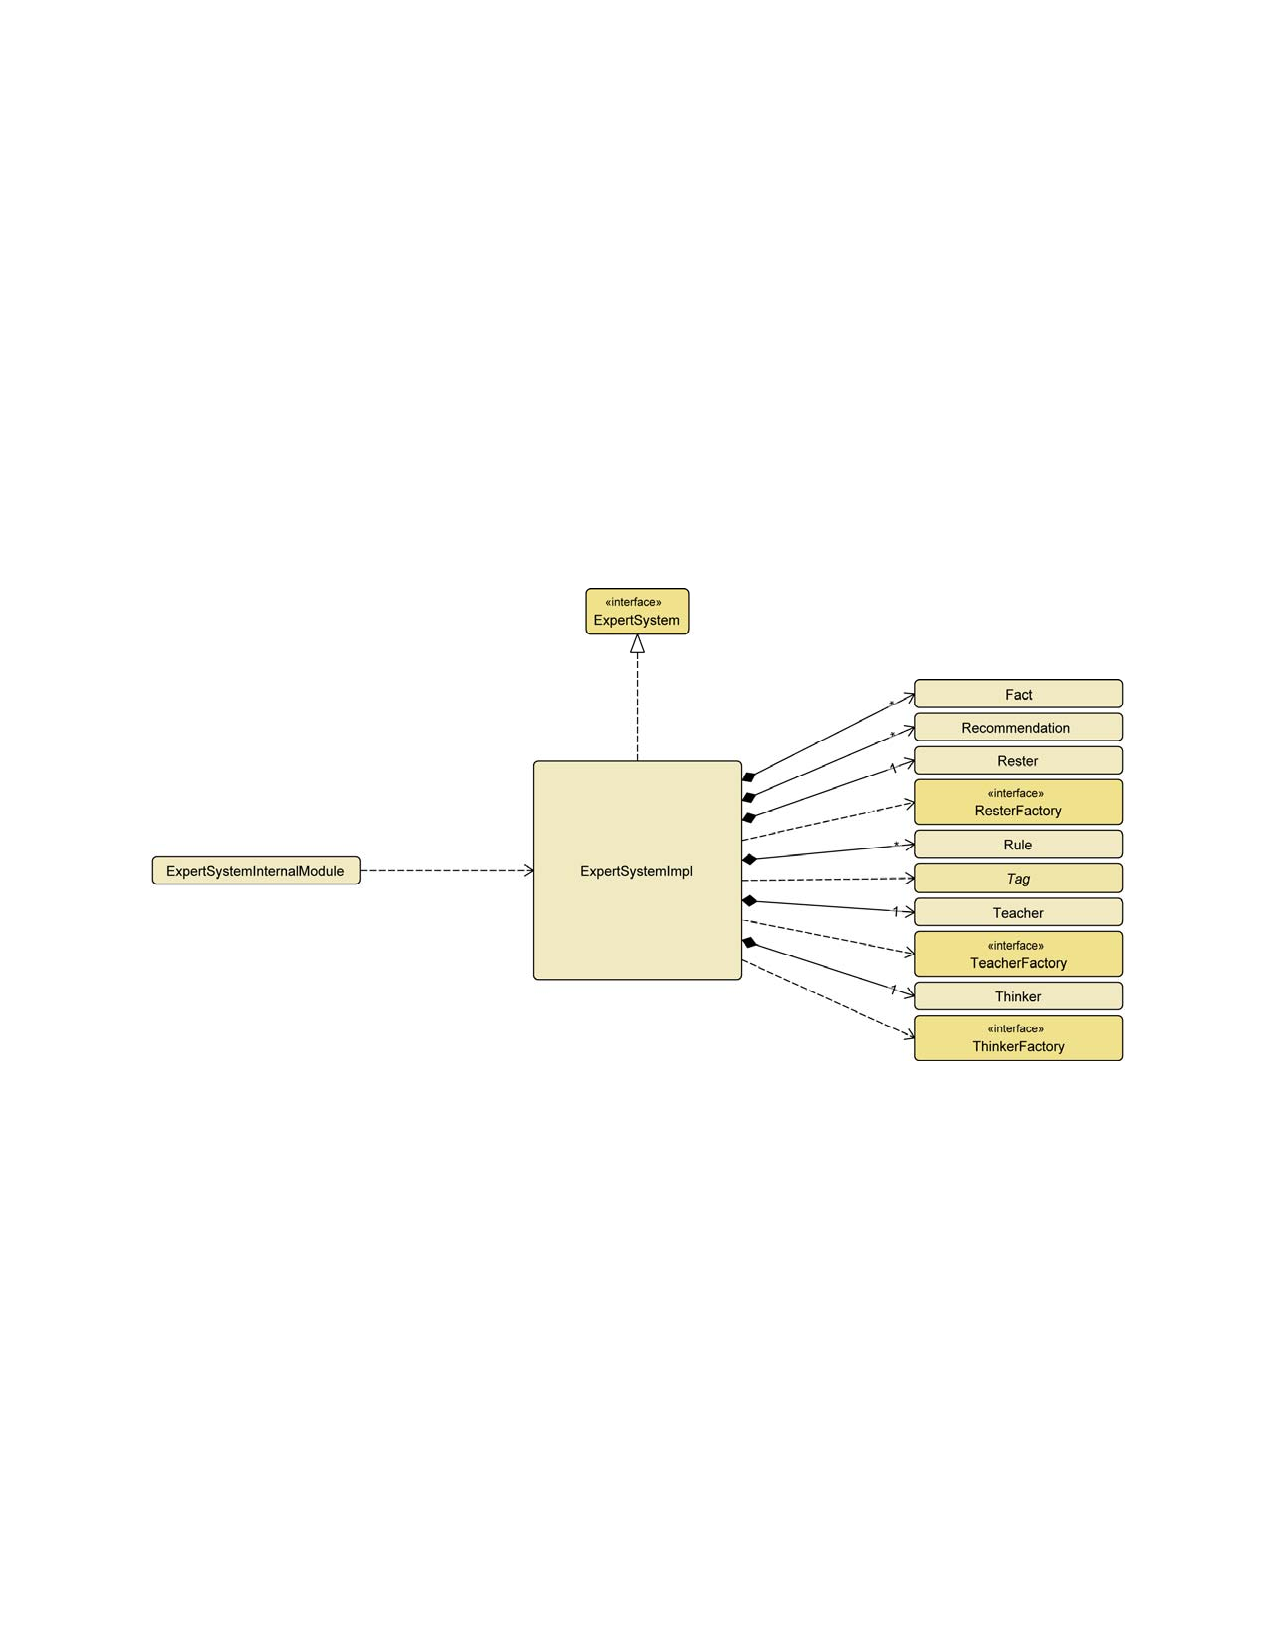
\includegraphics[width=\columnwidth]{figures/es_uml.pdf}
%							\caption
%							{ES package.}
%						\end{subfigure}
%						\begin{subfigure}[!htb]{0.4\columnwidth}
%							\centering
%							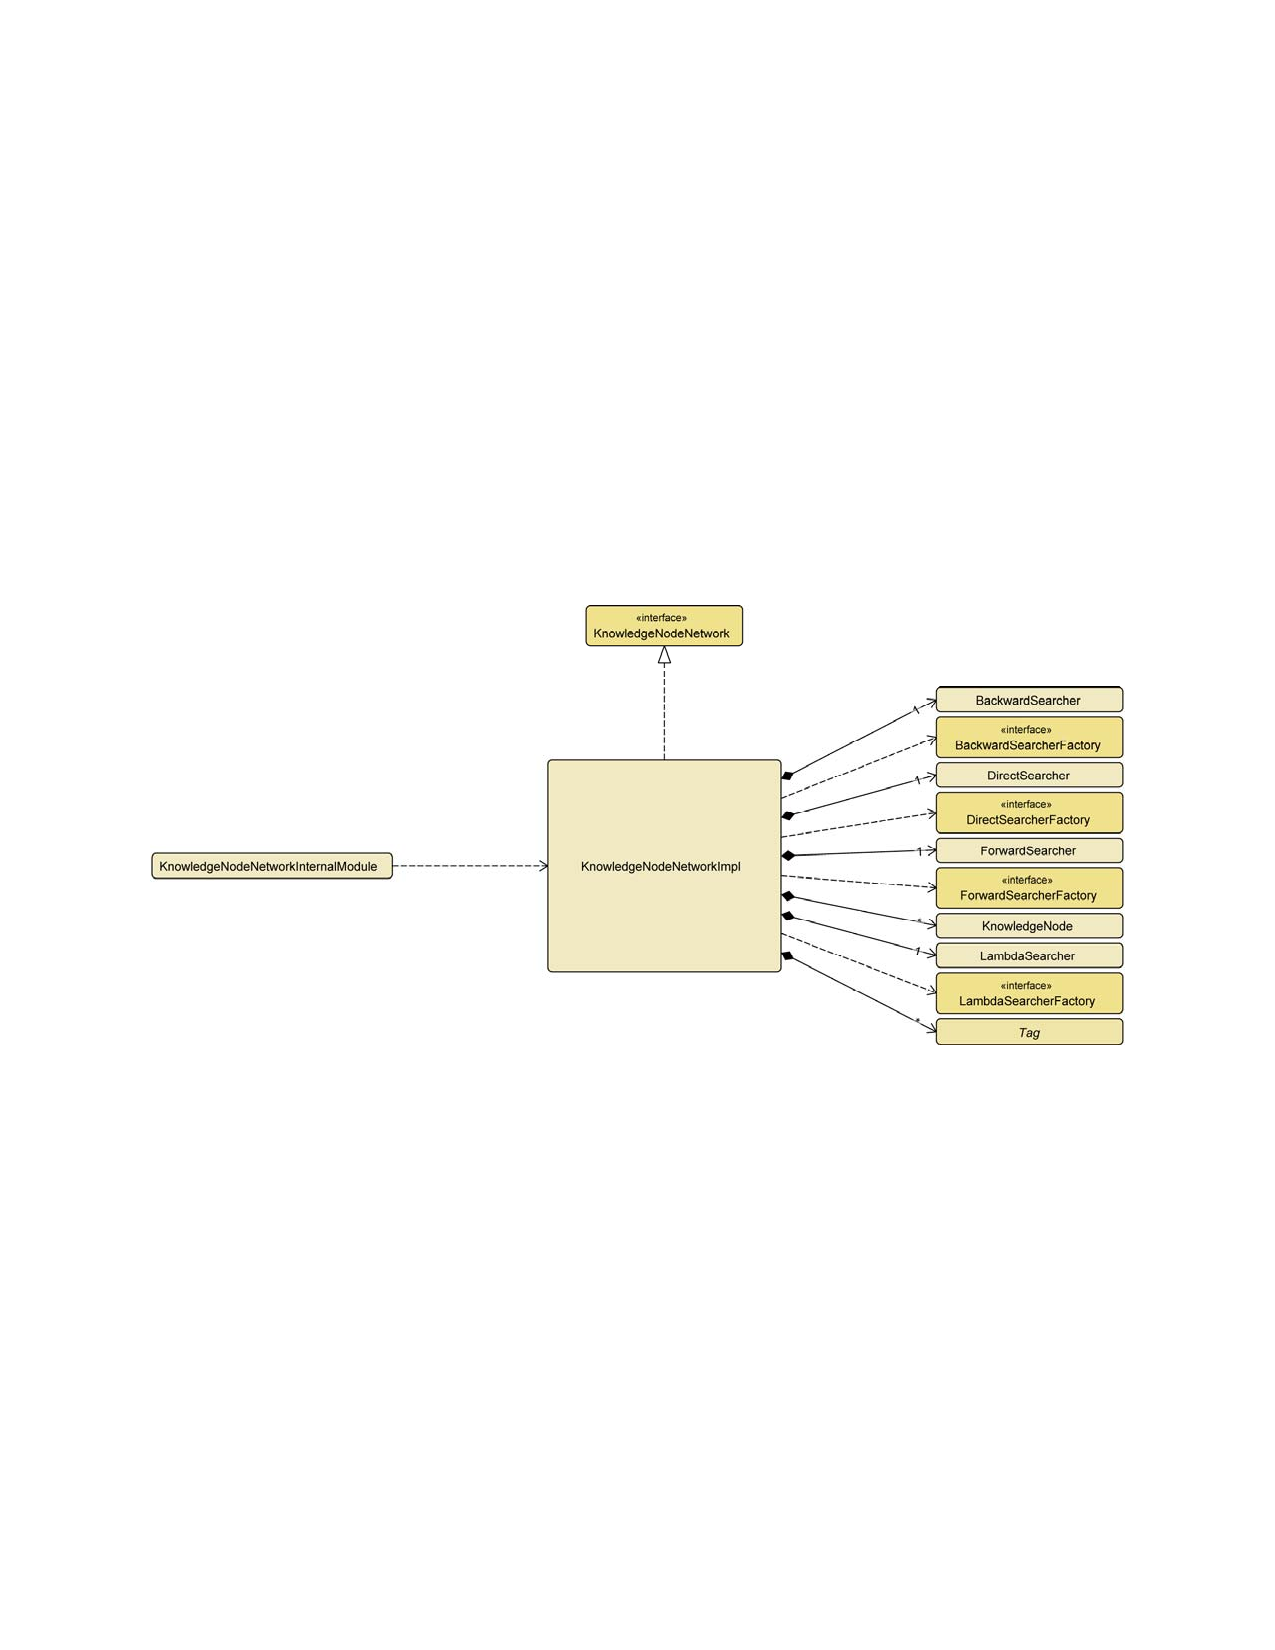
\includegraphics[width=\columnwidth]{figures/knn_uml.pdf}
%							\caption
%							{KNN package.}
%						\end{subfigure}
%						\caption{UML diagrams for the major modules.}
%					\end{figure}
					
%					\begin{figure}[!htb]
%						\centering
%						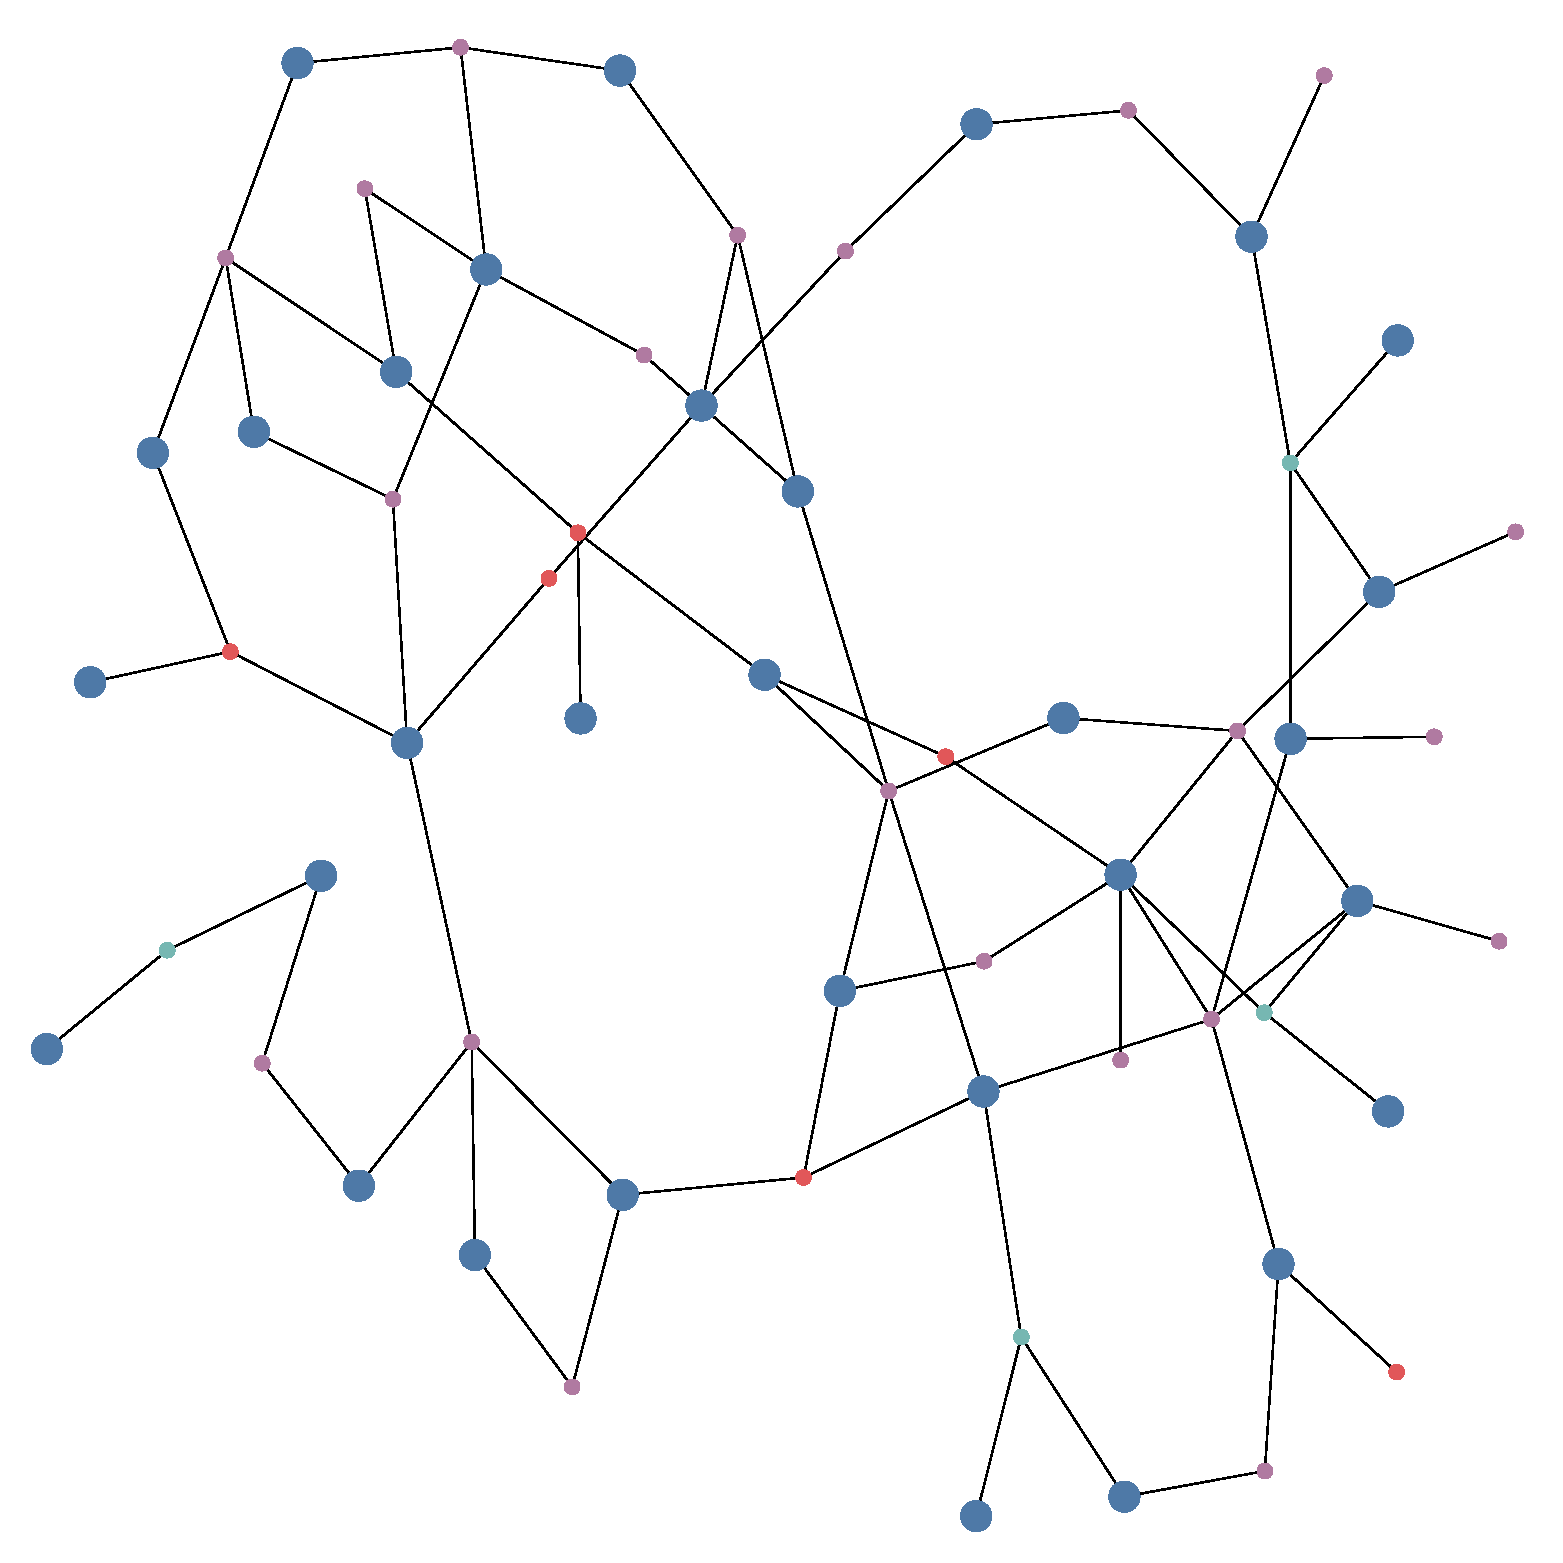
\includegraphics[width=0.3\columnwidth]{figures/knn_graph_svg.pdf}
%						\caption{Visualization of the KNN. Small nodes are Tags, big nodes are Knowledge Nodes (KNs). Red nodes represent active Tags or fired KNs. For non-active Tags, Facts are purple, Rules are blue and Recommendations are orange.}
%					\end{figure}
				\end{block}
				\begin{block}{Results \& Tests}
					\begin{itemize}
						\item Unit tests.
						\begin{itemize}
							\item Testing individual methods of every class in the KNN and ES.
							\item Dependencies mocked using the Mockito library.
						\end{itemize}
					\end{itemize}
					
					\begin{itemize}
						\item Integration tests.
						\begin{itemize}
							\item Testing end-to-end behavior of the ES and KNN modules.
							\item All unit and integration tests written with TestNG and executed with TravisCI.
						\end{itemize}
					\end{itemize}
				
					\begin{figure}[!htb]
						\centering
						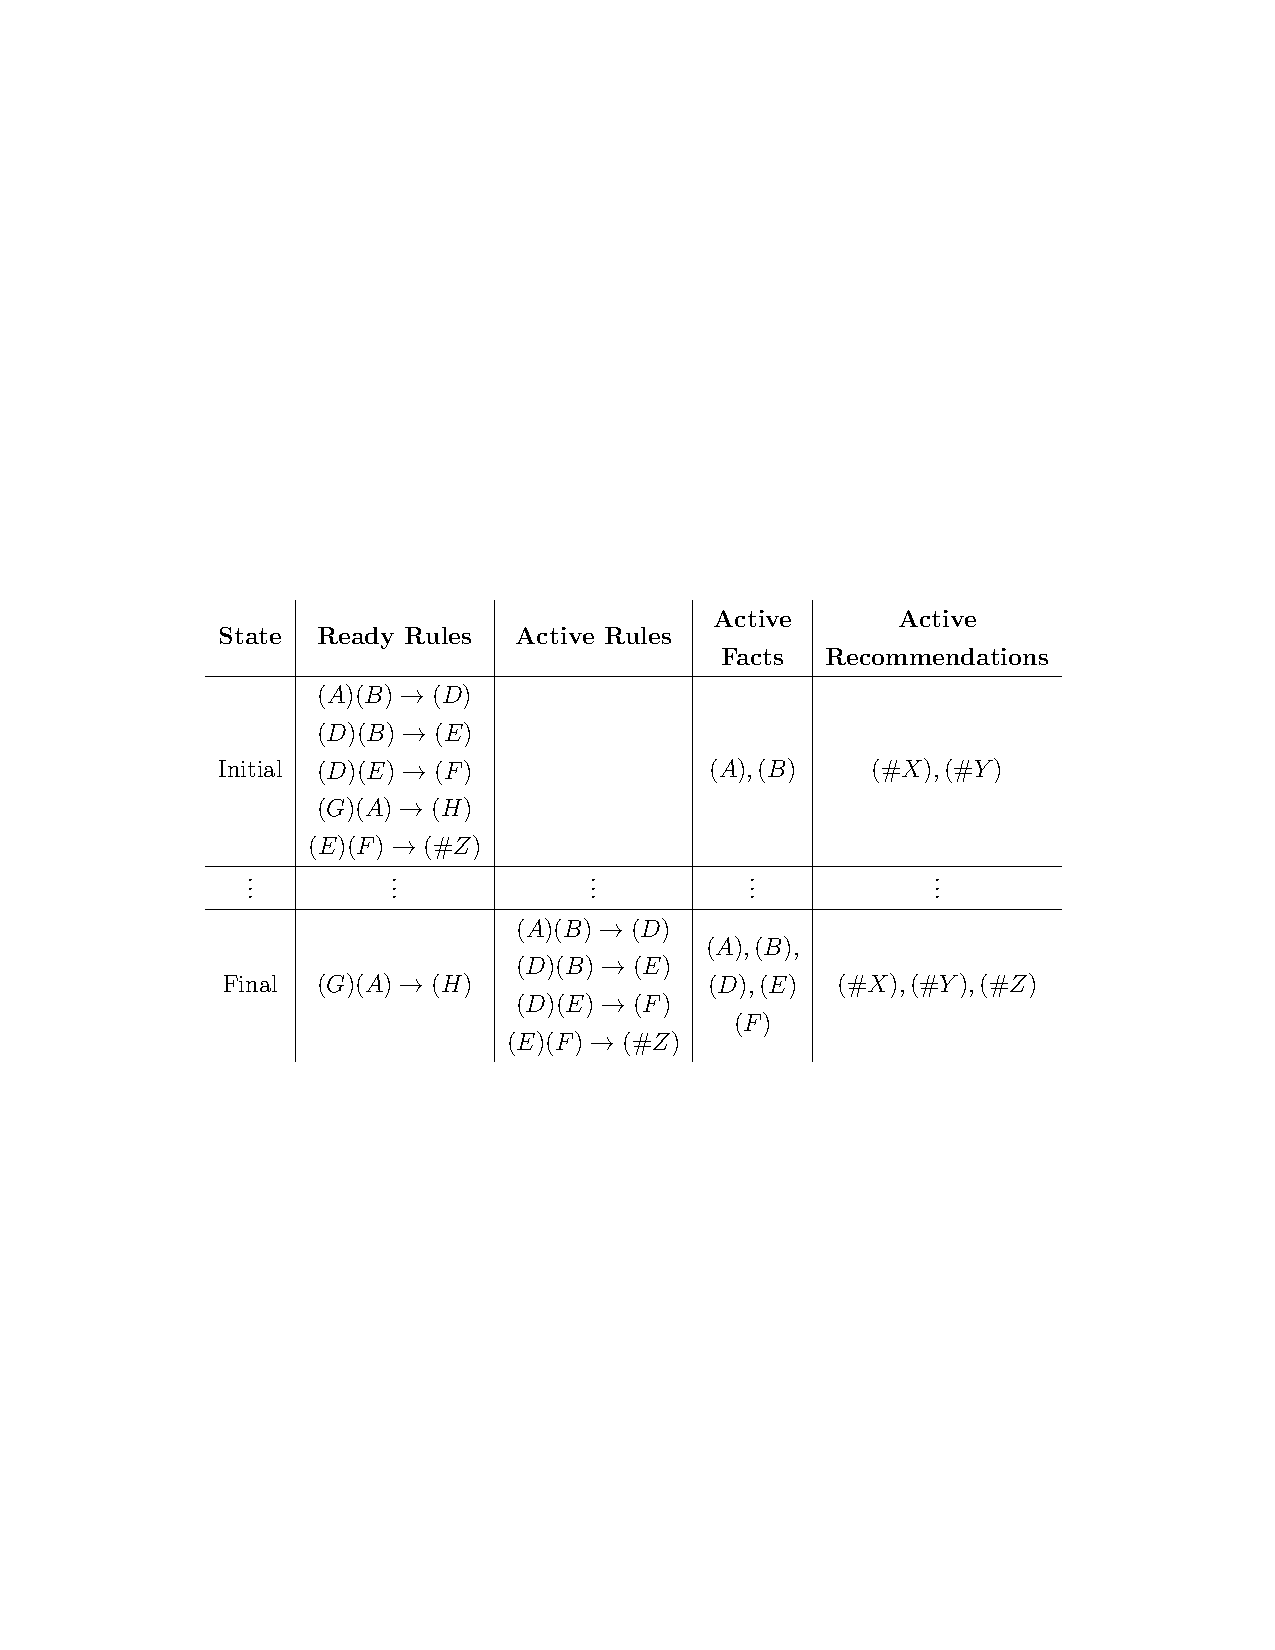
\includegraphics[width=0.7\textwidth]{figures/testES.pdf}
						\caption
						{ES test setup representing simple rules and facts that must be brought to quiescence.}
					\end{figure}
				\end{block}
				}
			\end{column}
			\begin{column}{.3\textwidth}
				\parbox[t][\columnheight]{\textwidth}{
				\begin{block}{Results \& Tests (continued)}
					\begin{figure}[!htb]
						\centering
						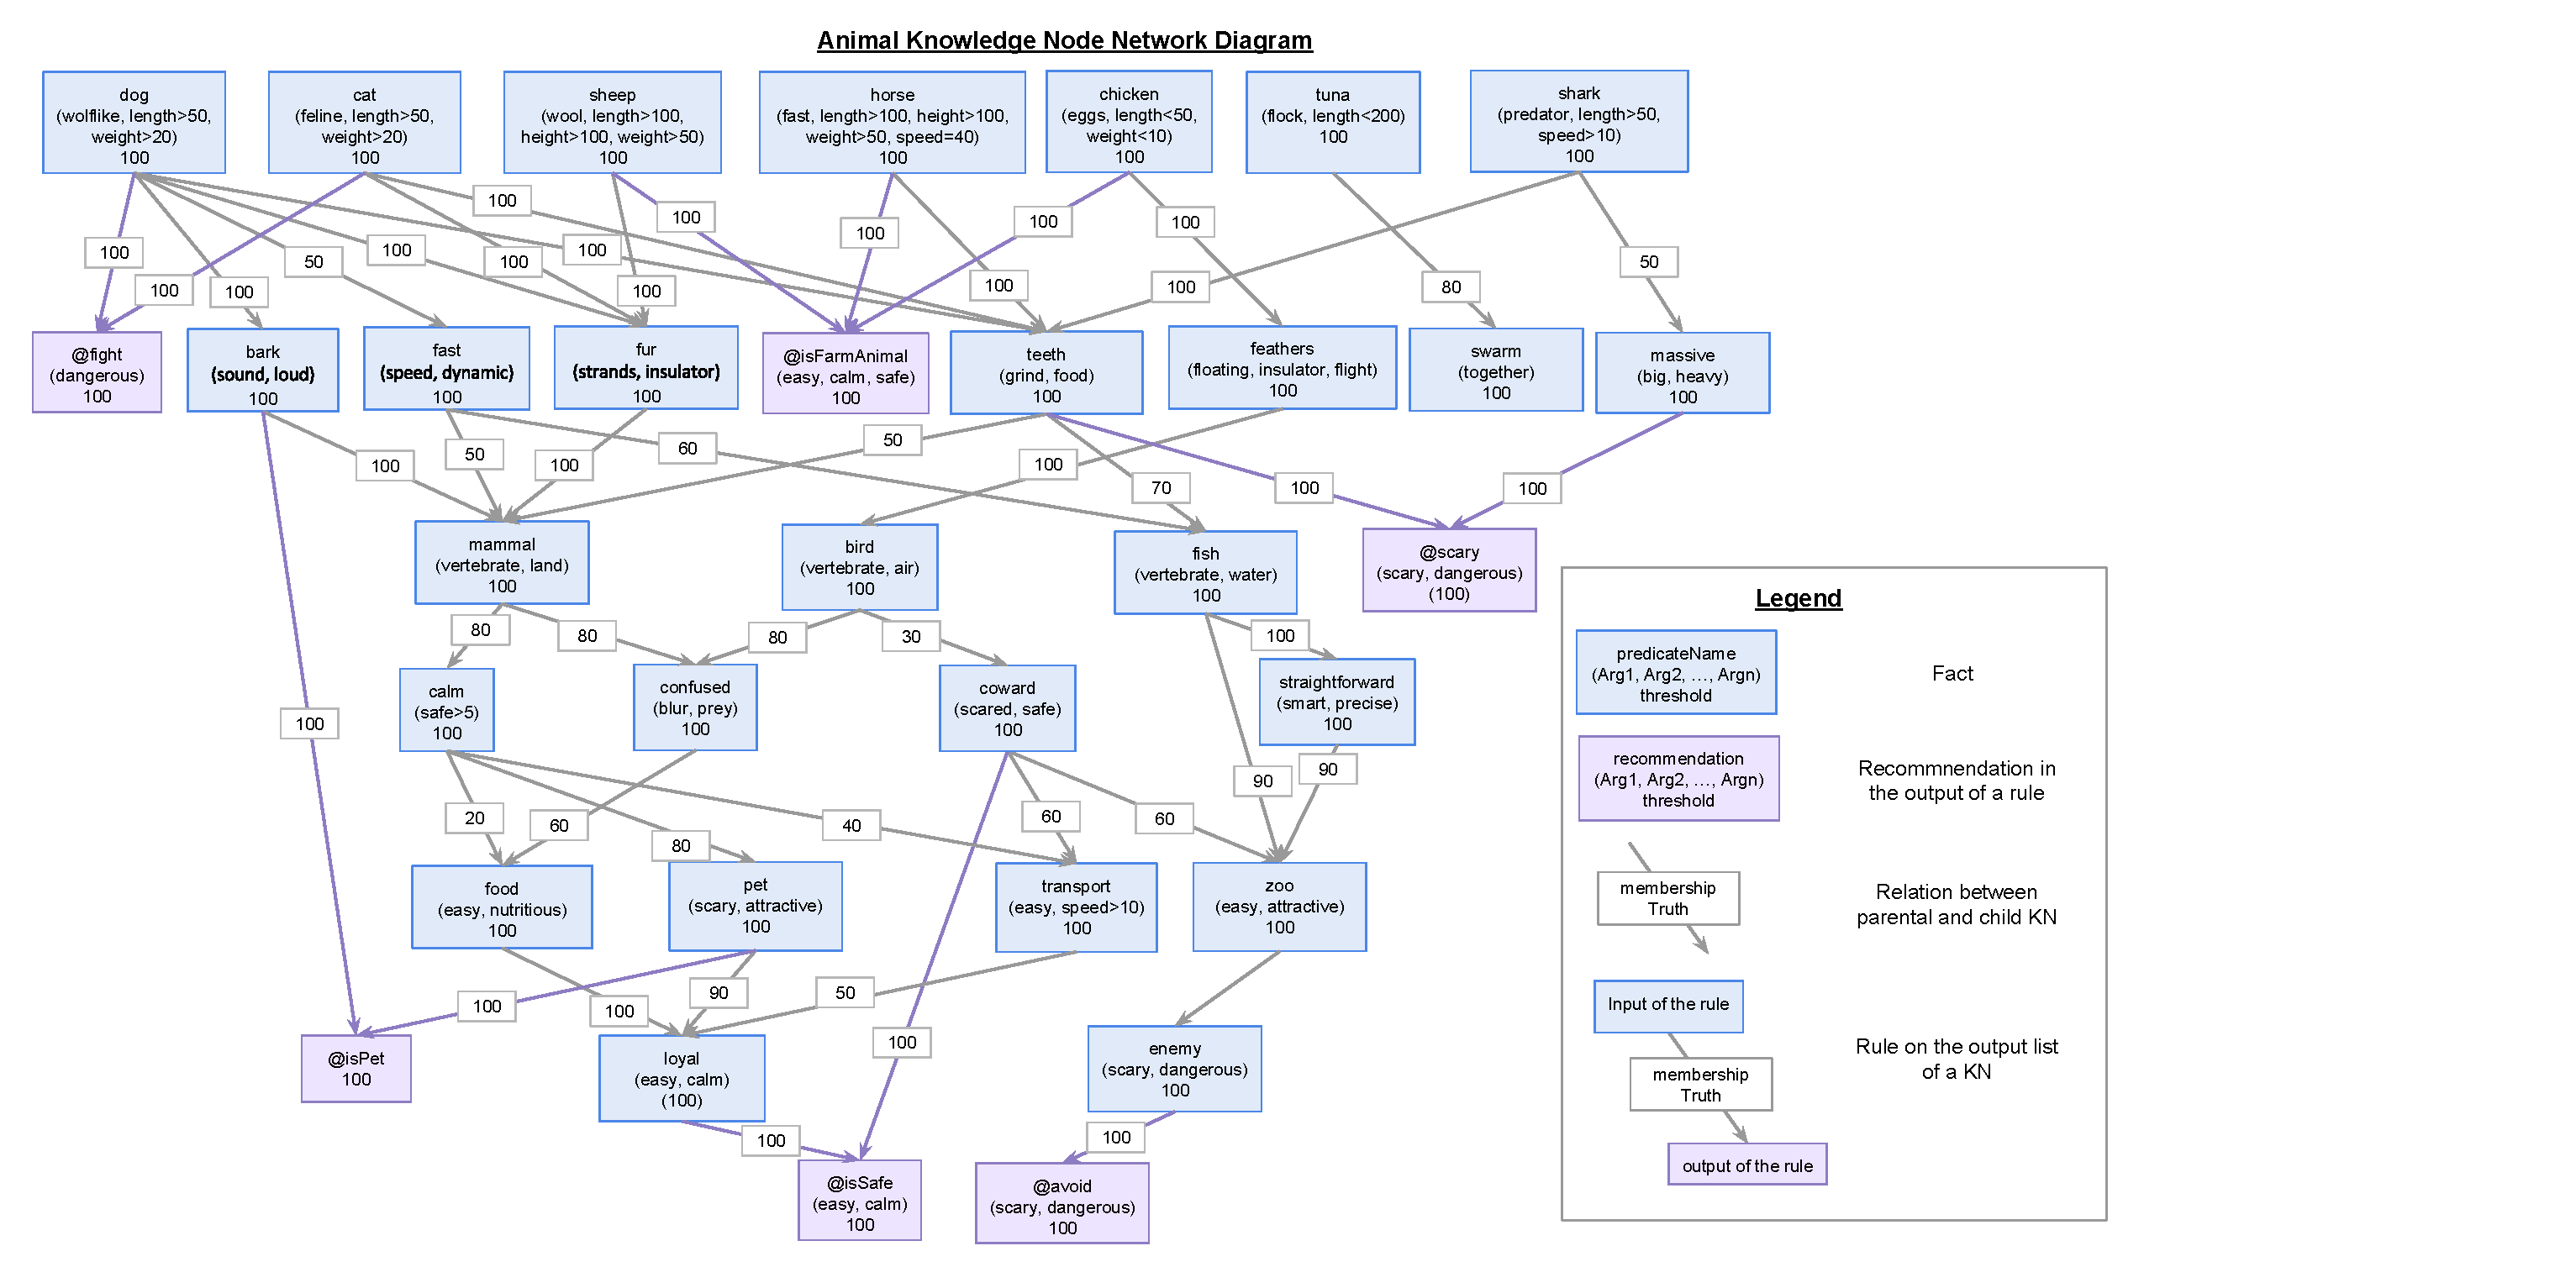
\includegraphics[width=\textwidth]{figures/animal_knn.pdf}
						\caption
						{Elaborate test KNN network representing connections between memories of animals and their characteristics.}
					\end{figure}
					
					\begin{itemize}
						\item Graph visualization tests.
						\begin{itemize}
							\item Iterations of the KNN searching algorithms are presented visually.
						\end{itemize}
					\end{itemize}
					
					\begin{figure}[!htb]
						\centering
						\begin{subfigure}[!htb]{0.24\columnwidth}
							\centering
							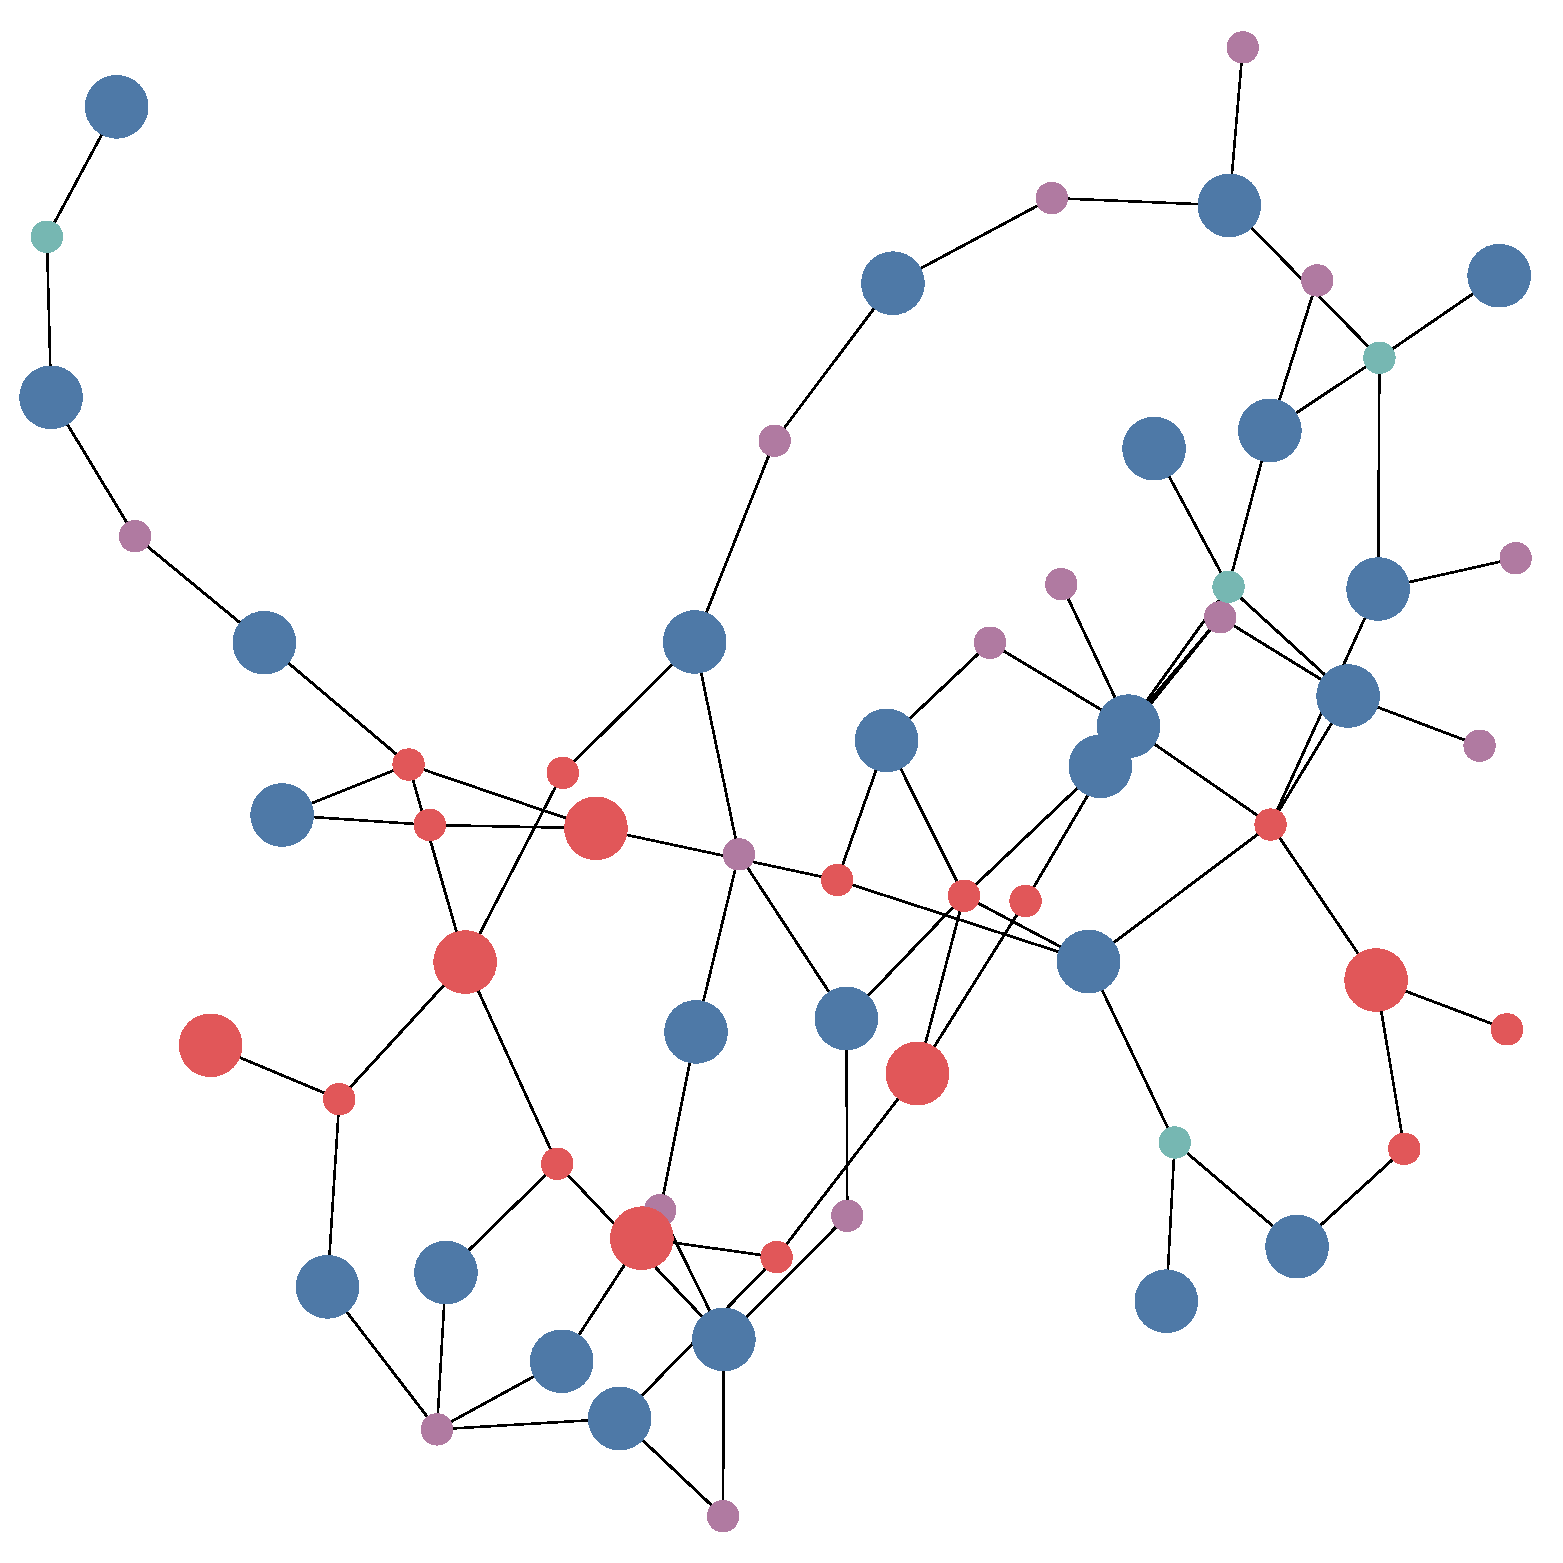
\includegraphics[width=\columnwidth]{figures/knn_forward_think_1.pdf}
							\caption{Ply 1.}
						\end{subfigure}
						\begin{subfigure}[!htb]{0.24\columnwidth}
							\centering
							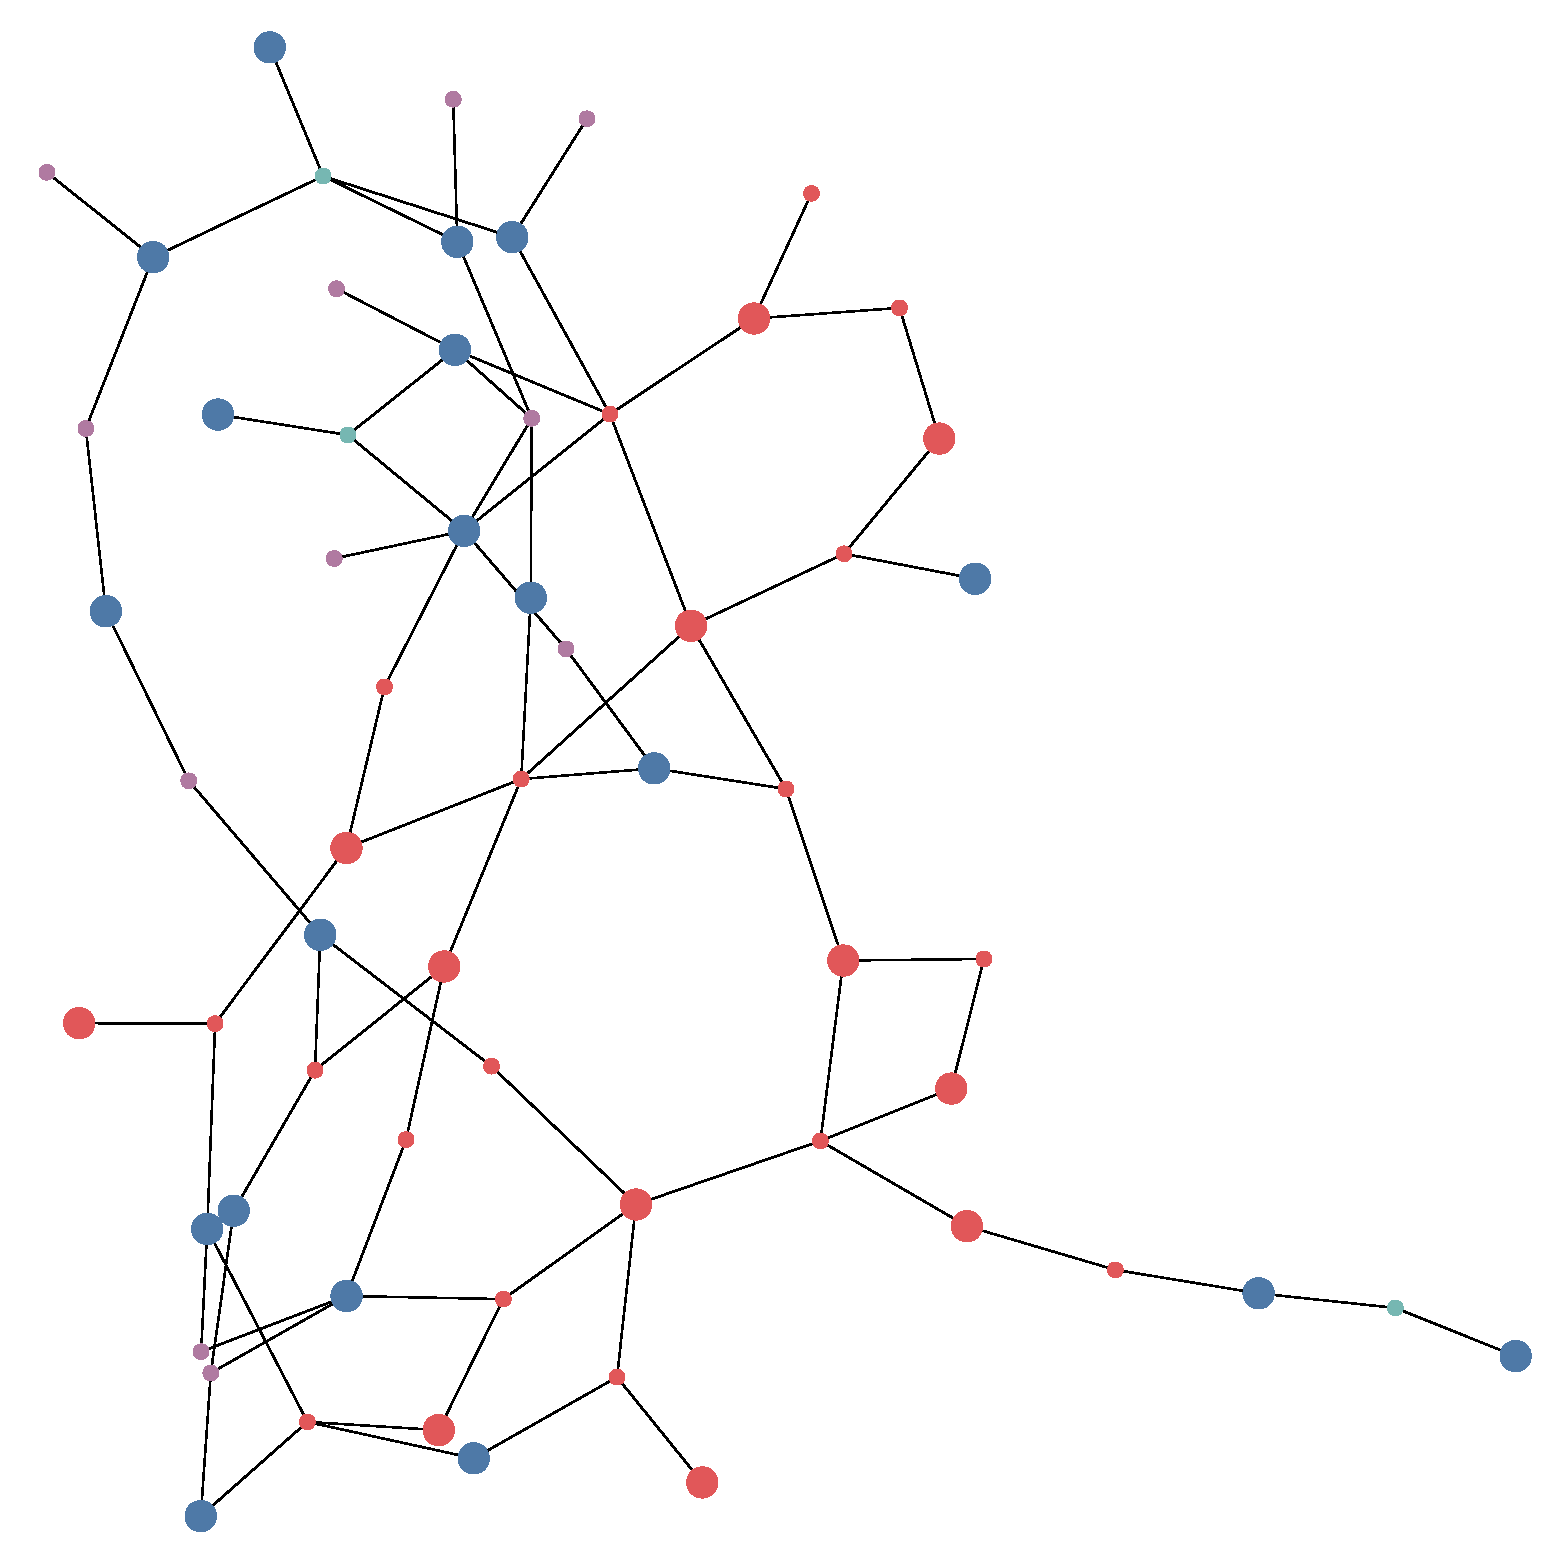
\includegraphics[width=\columnwidth]{figures/knn_forward_think_2.pdf}
							\caption{Ply 2.}
						\end{subfigure}
						\begin{subfigure}[!htb]{0.24\columnwidth}
							\centering
							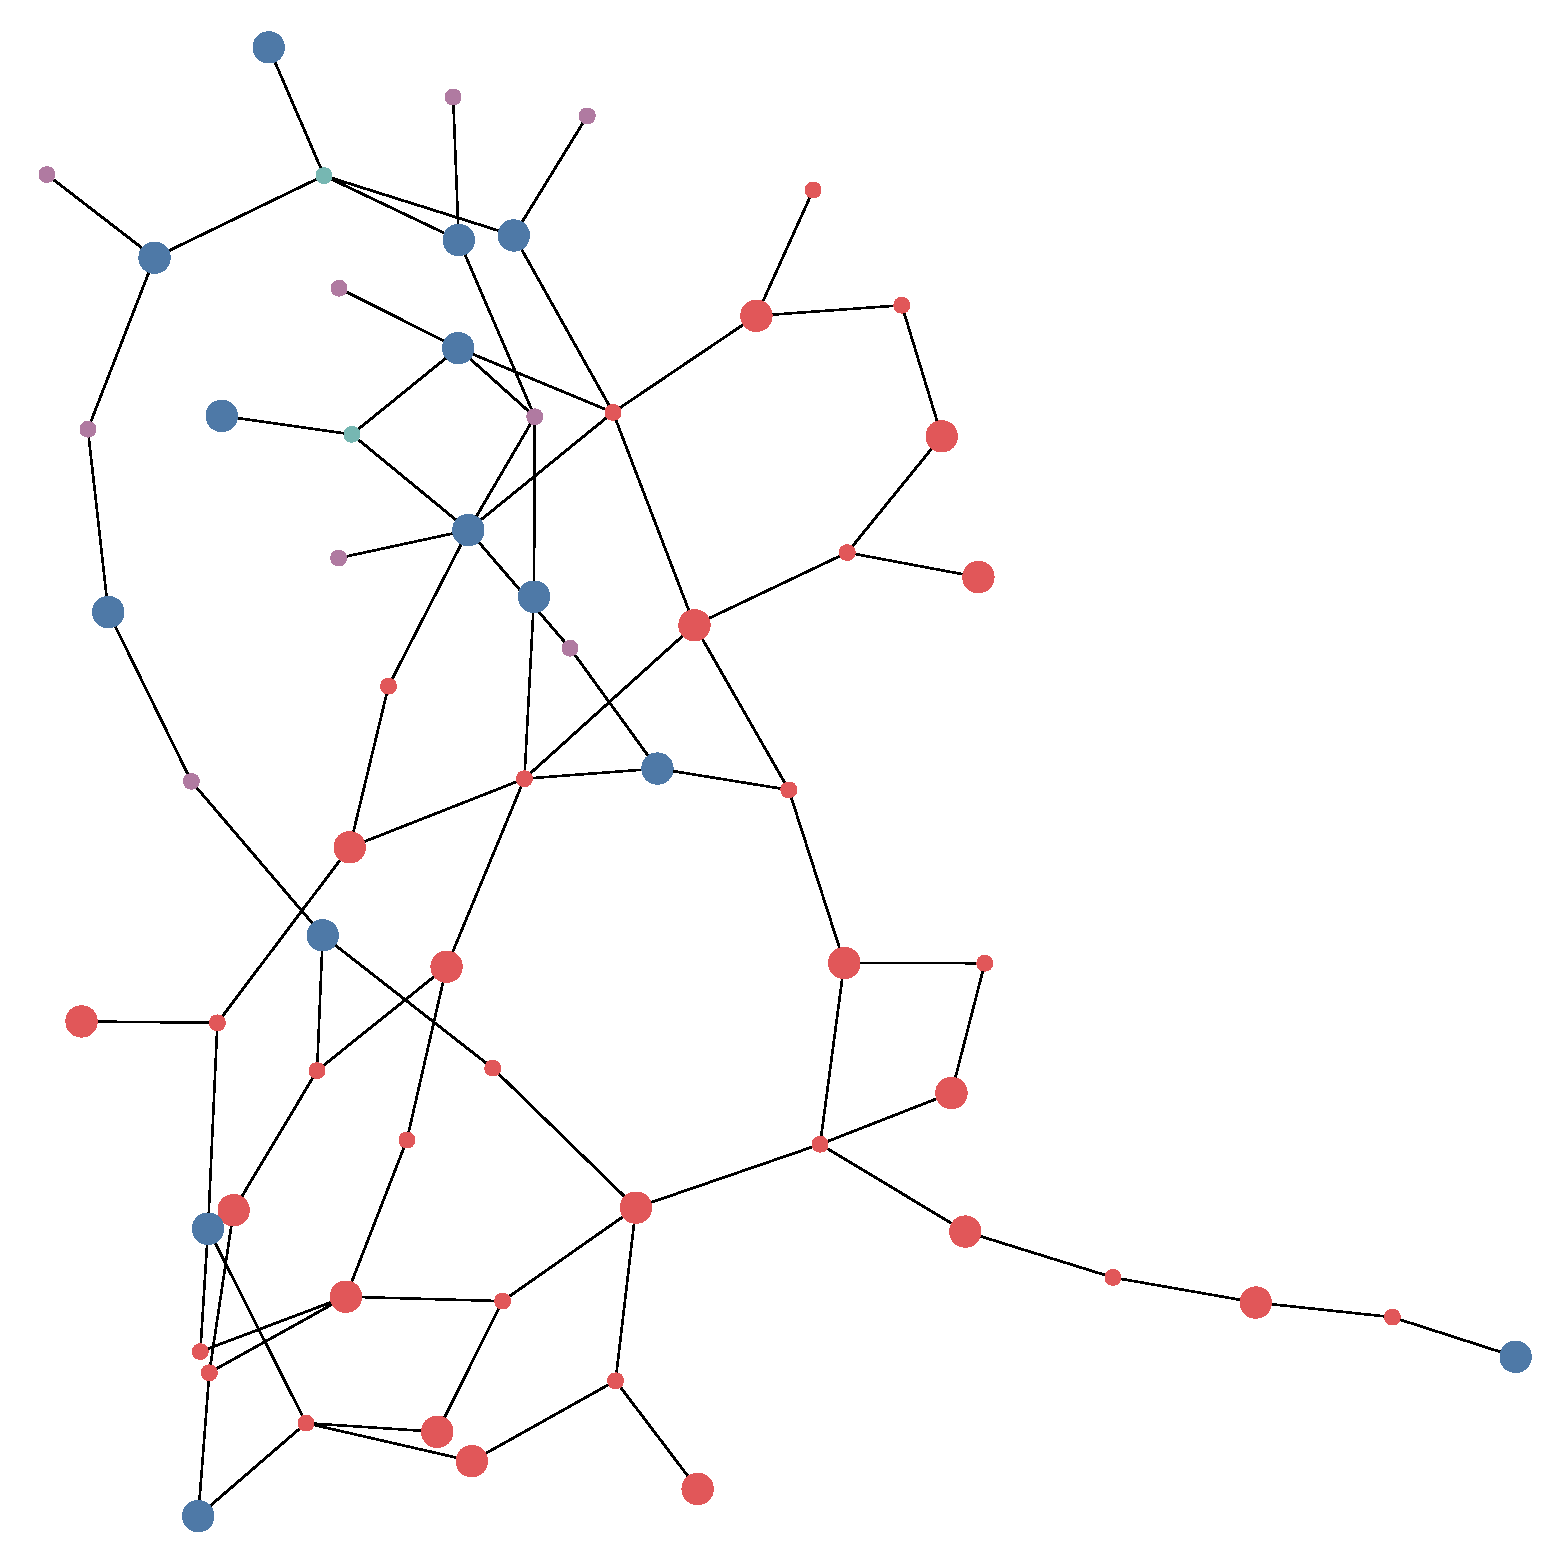
\includegraphics[width=\columnwidth]{figures/knn_forward_think_3.pdf}
							\caption{Ply 3.}
						\end{subfigure}
						\begin{subfigure}[!htb]{0.24\columnwidth}
							\centering
							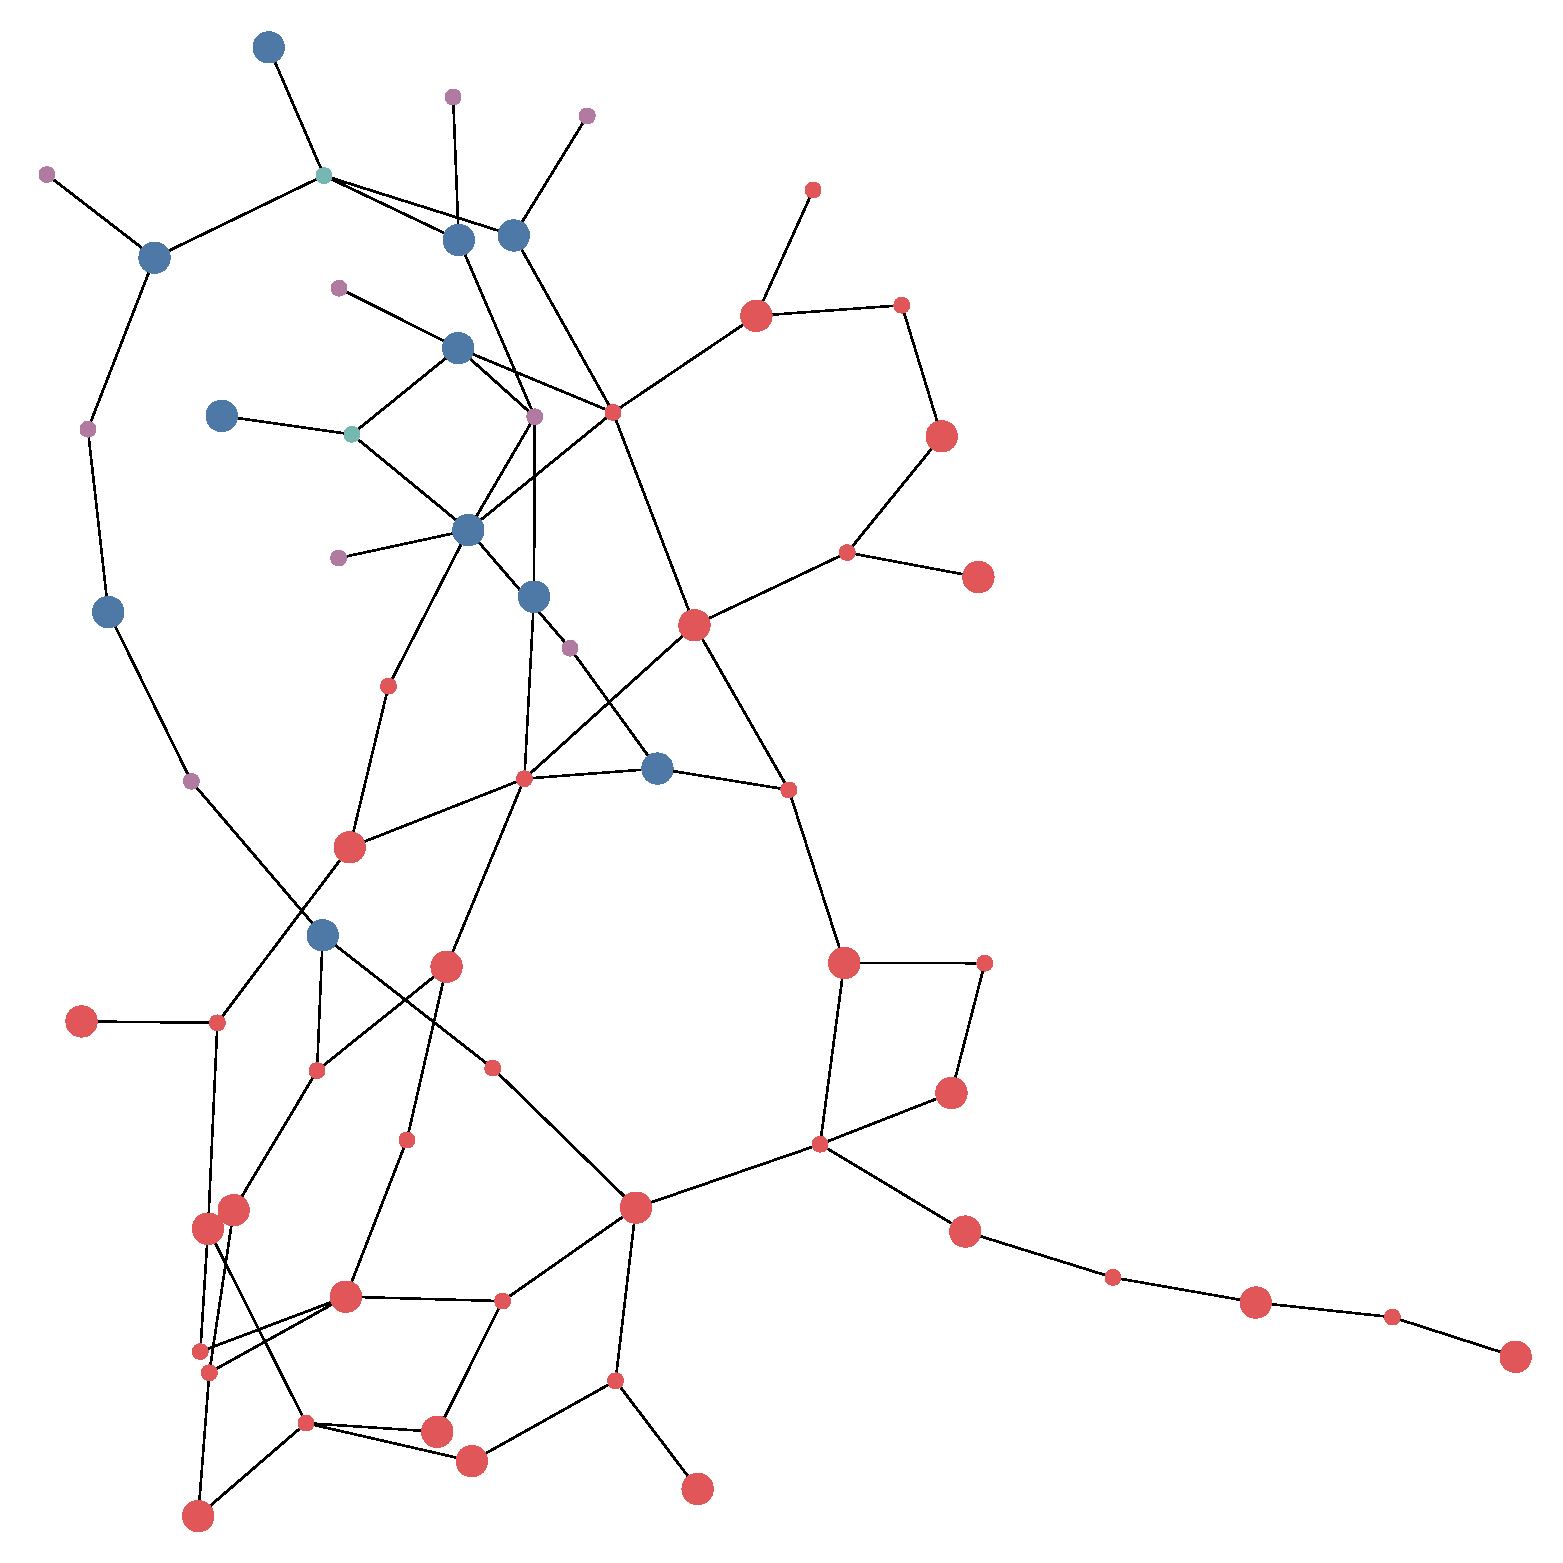
\includegraphics[width=\columnwidth]{figures/knn_forward_think_4.pdf}
							\caption{Ply 4.}
						\end{subfigure}
						\caption{Forward thinking visualization in the KNN.}
					\end{figure}
					
					\begin{figure}[!htb]
						\centering
						\begin{subfigure}[!htb]{0.24\columnwidth}
							\centering
							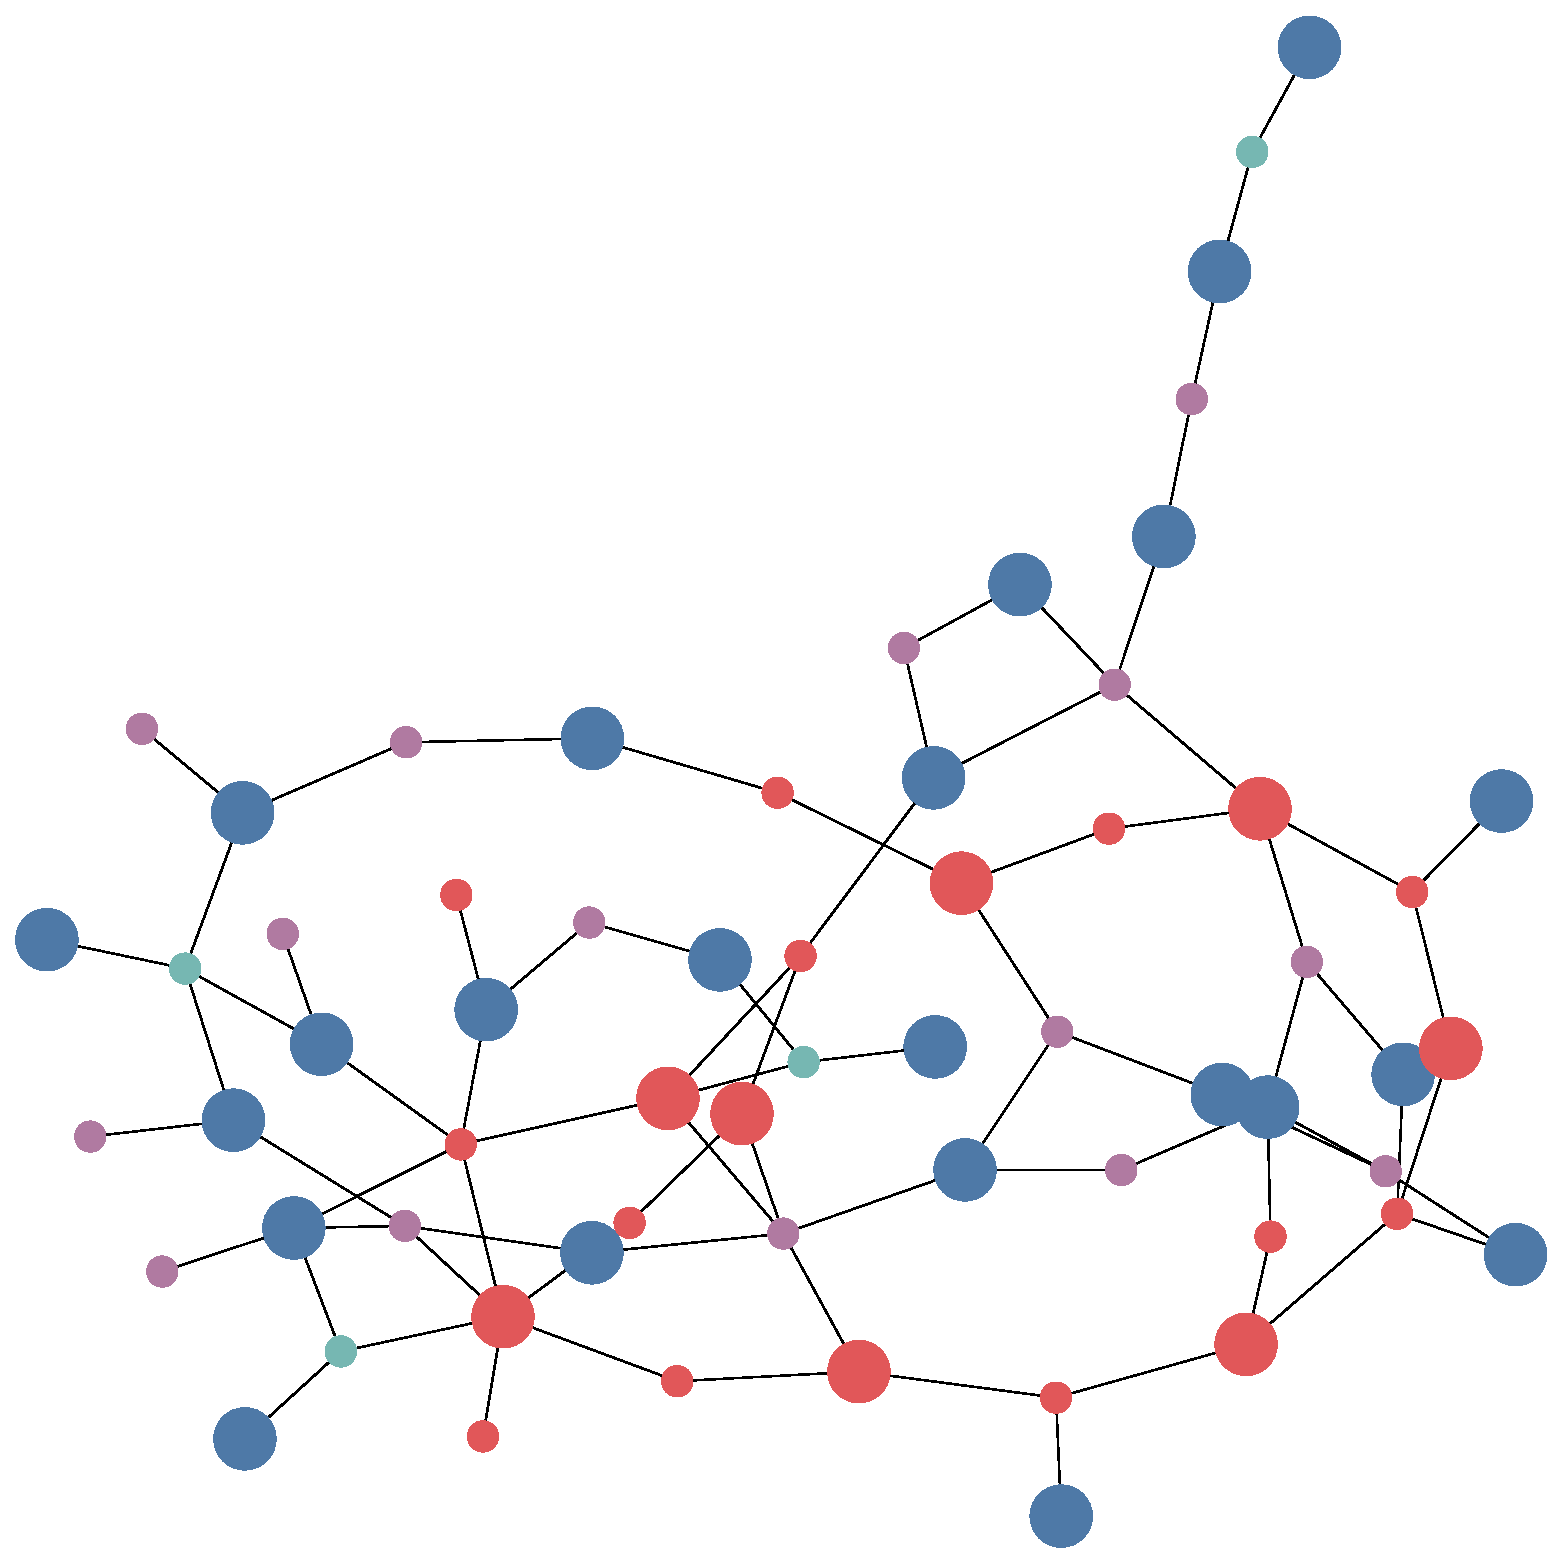
\includegraphics[width=\columnwidth]{figures/knn_backward_think_1.pdf}
							\caption{Ply 1.}
						\end{subfigure}
						\begin{subfigure}[!htb]{0.24\columnwidth}
							\centering
							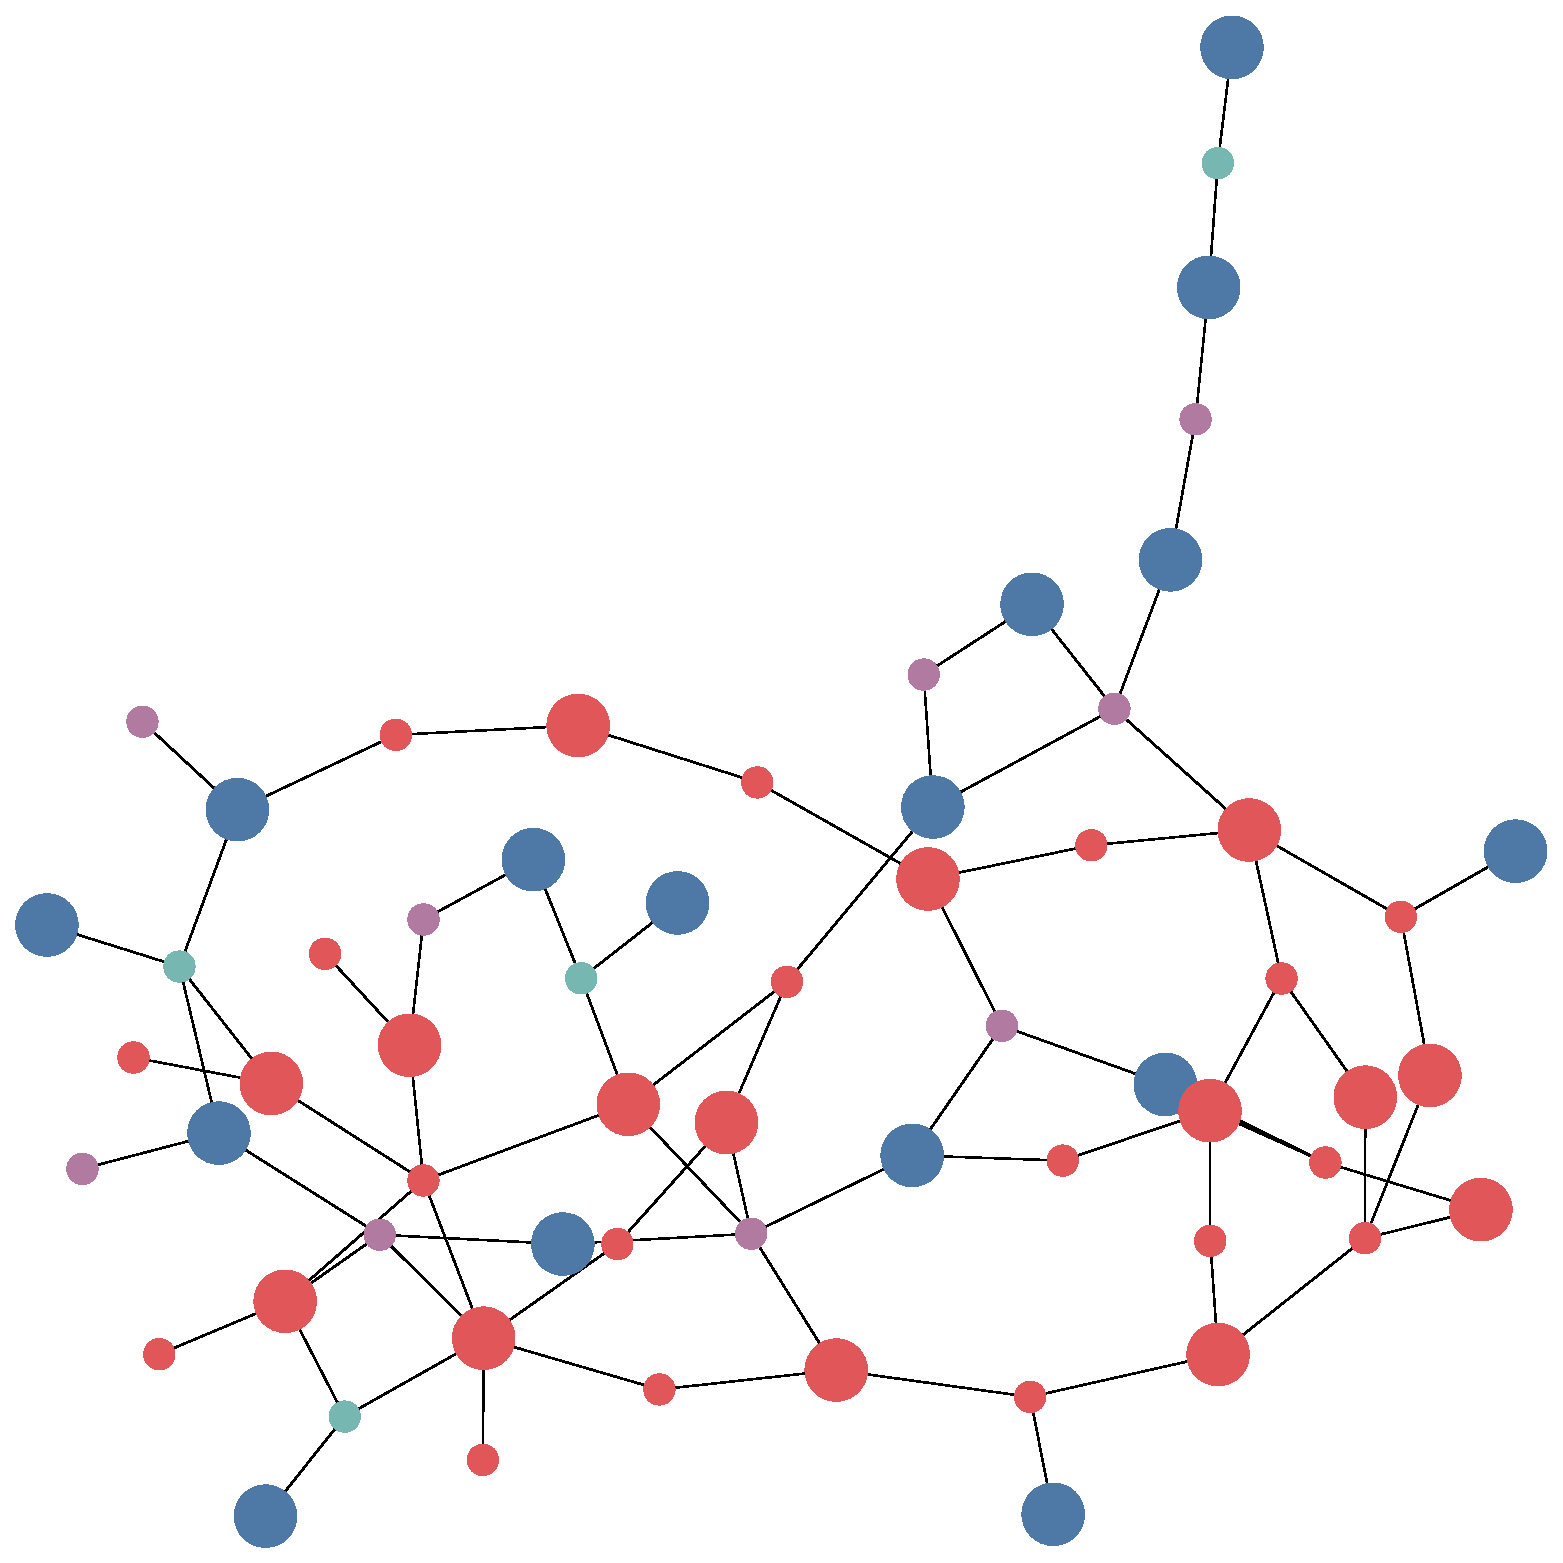
\includegraphics[width=\columnwidth]{figures/knn_backward_think_2.pdf}
							\caption{Ply 2.}
						\end{subfigure}
						\begin{subfigure}[!htb]{0.24\columnwidth}
							\centering
							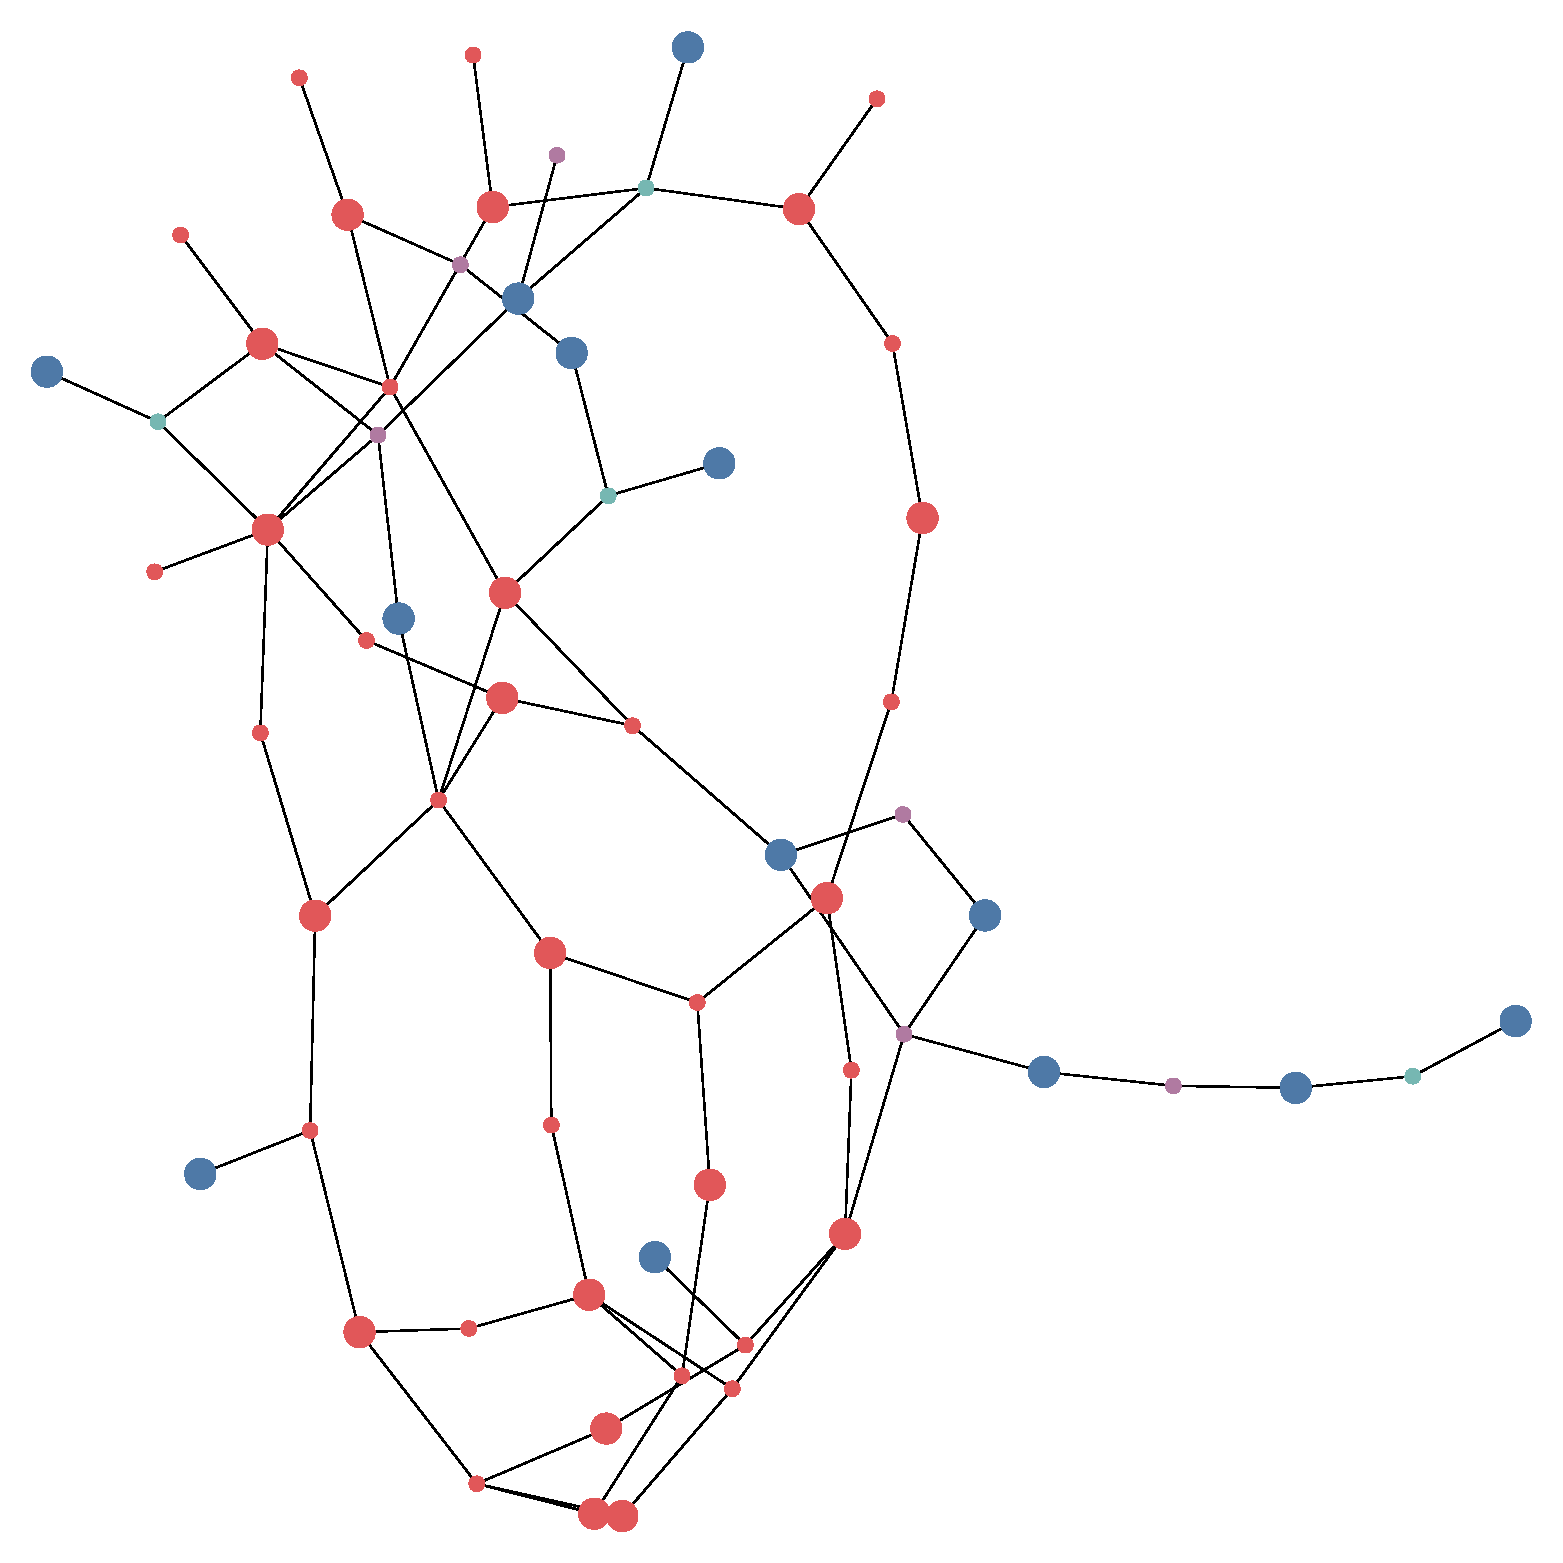
\includegraphics[width=\columnwidth]{figures/knn_backward_think_3.pdf}
							\caption{Ply 3.}
						\end{subfigure}
						\begin{subfigure}[!htb]{0.24\columnwidth}
							\centering
							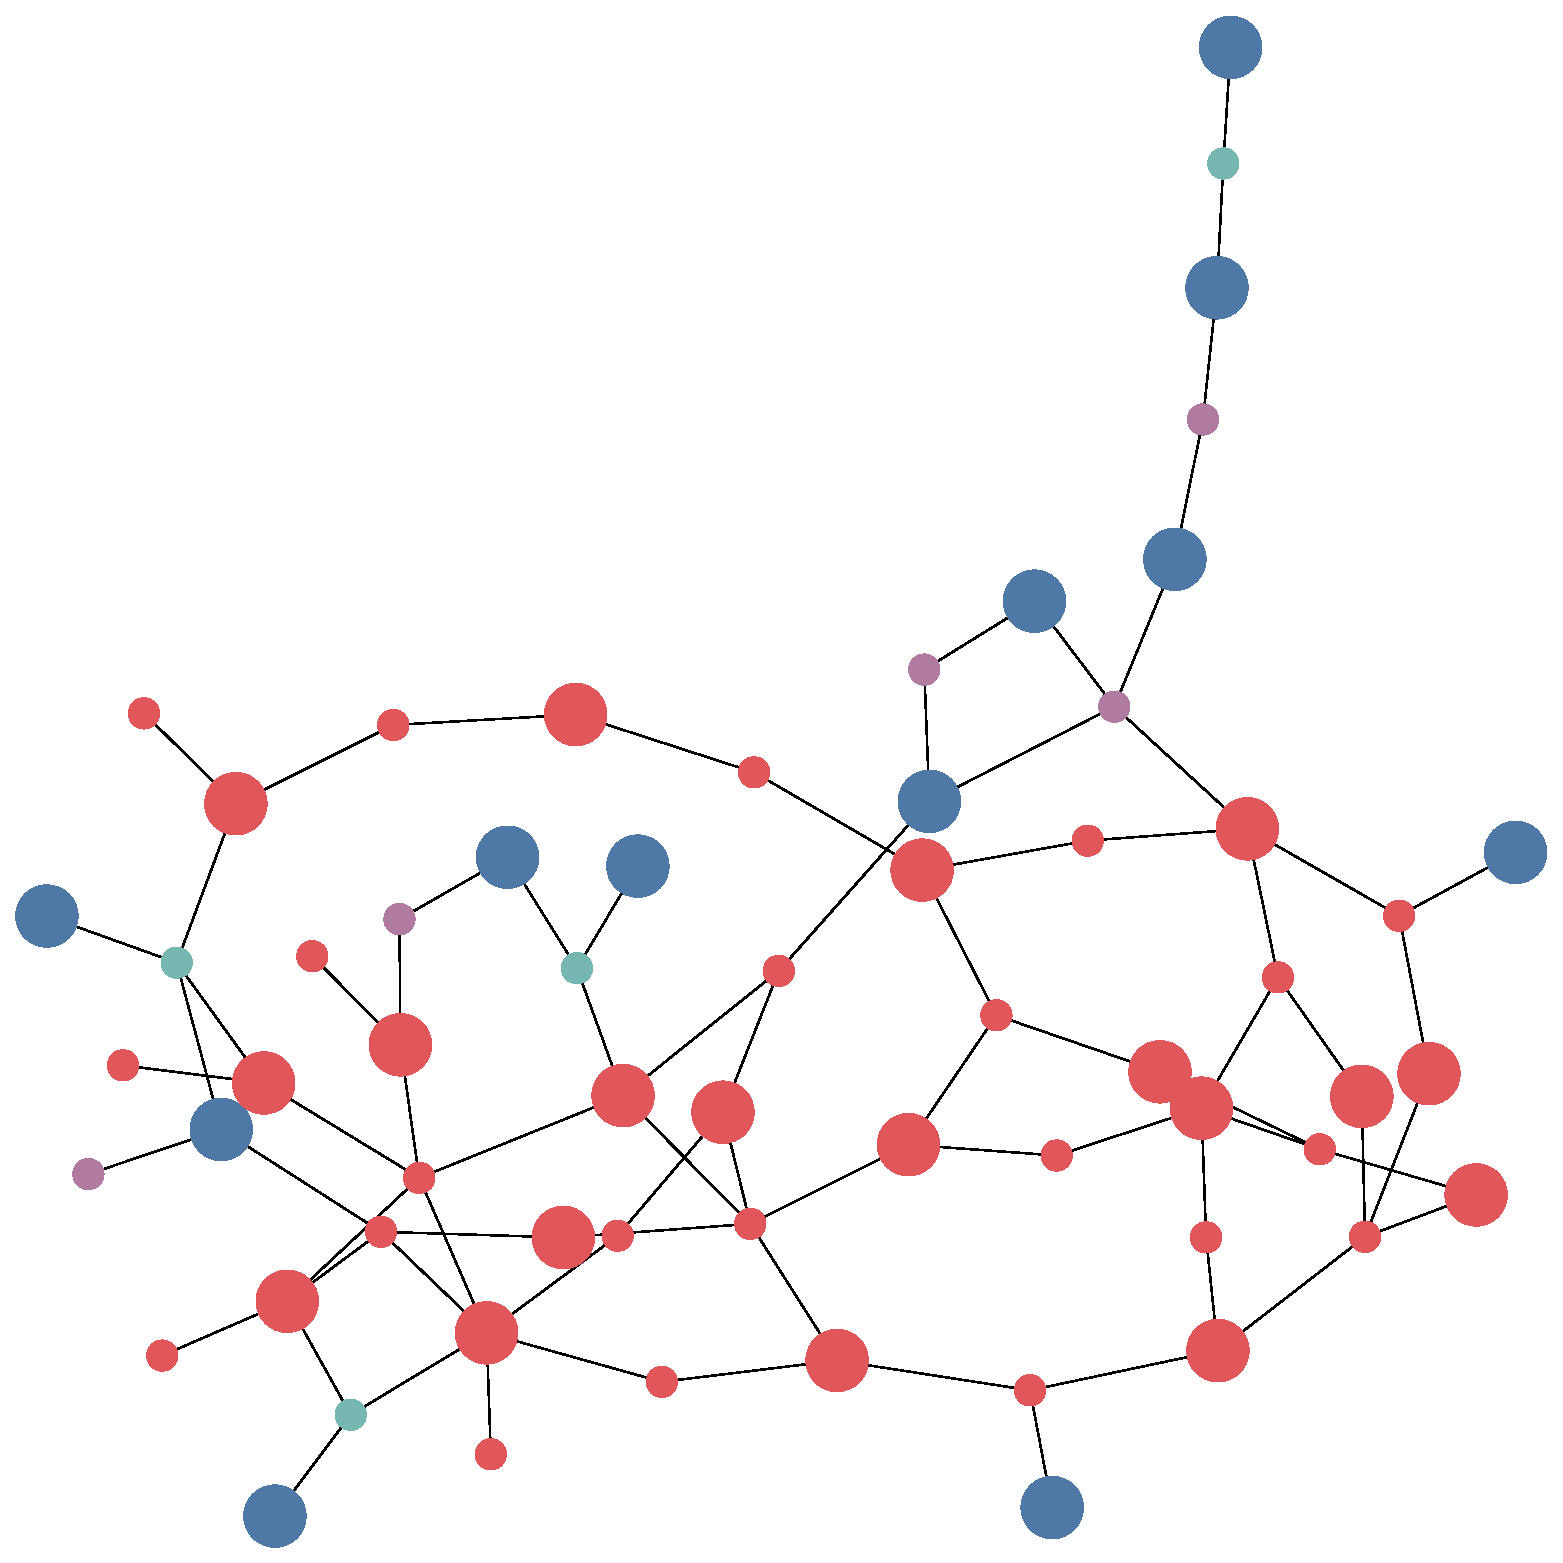
\includegraphics[width=\columnwidth]{figures/knn_backward_think_4.pdf}
							\caption{Ply 4.}
						\end{subfigure}
						\caption{Backward thinking visualization in the KNN.}
					\end{figure}
				\end{block}
				\begin{block}{Conclusion}
					\begin{itemize}
						\item Skills learned:
						\begin{itemize}
							\item Planning and implementing large software project.
							\item Time management.
							\item People management.
						\end{itemize}
					
						\item Possible future work:
						\begin{itemize}
							\item Implement the missing NN and META layers.
							\item Explore further features in the KNN, such as learning and attention.
						\end{itemize}
					\end{itemize}
				\end{block}
			}
			\end{column}
		\end{columns}
	\end{frame}
\end{document}